\chapter{Estrutura do Template}

O template TED ITA-SAC foi organizado de forma modular, para facilitar manutenção, reuso e colaboração entre diferentes autores. A estrutura principal está organizada da seguinte forma:

\section{Visão geral}

\begin{verbatim}
	.
	|- main.tex                 % Arquivo principal (documento raiz)
	|- settings/                % Configurações gerais
	|  |- background.tex        % Marca d’água e fundo
	|  |- coverpage.tex         % Página de capa
	|  |- fonts.tex             % Fonte Cheltenham
	|  |- pretextualpages.tex  % Sumário, listas, elementos iniciais
	|  |- setabnt.tex          % Estilo de citação ABNT
	|  |- setcolor.tex         % Paleta de cores do template
	|  |- setlayout.tex        % Margens, espaçamento, cabeçalho
	|  |- settitles.tex        % Estilo de títulos e capítulos
	|  \_ usepackage.tex       % Pacotes utilizados no projeto
	|- caps/                   % Capítulos do relatório
	|  |- cap00.tex            % Introdução
	|  |- cap01.tex            % Conteúdo específico
	|  \_ etc.
	|- siglas/                 % (Opcional) Siglas, glossários
	|- refs/                   % (Opcional) Arquivos .bib
	\_ Makefile                % Automação de compilação
\end{verbatim}


\section{Função de cada componente}

\begin{itemize}
    \item \texttt{main.tex}: ponto de entrada do projeto. Controla a ordem dos elementos.
    \item \texttt{settings/}: conjunto de arquivos para configurar todos os aspectos do template.
    \item \texttt{caps/}: contém os capítulos do relatório (modularizados).
    \item \texttt{siglas/}: pasta destinada ao glossário e acrônimos, caso ativado.
    \item \texttt{refs/}: local sugerido para o arquivo de bibliografia (\texttt{.bib}).
    \item \texttt{Makefile}: automatiza as etapas de compilação (XeLaTeX + BibTeX + Glossário).
\end{itemize}

\section{Ordem de carregamento no \texttt{main.tex}}

O arquivo \texttt{main.tex} importa os componentes da seguinte forma:

\begin{verbatim}
% defs_setusepackage.tex
% --- PACOTES DO TEMPLATE AIRDATA ---


% --- Tipografia e fontes ---
\usepackage{fontspec}       % Uso de fontes OpenType com XeLaTeX

% --- Cores institucionais ---
\usepackage{xcolor}         % Suporte a cores em HTML, RGB etc.

% --- Gráficos e imagens ---
\usepackage{graphicx}       % Inclusão de imagens (.png, .pdf etc.)
\usepackage{eso-pic}        % Permite inserir elementos em todas as páginas (fundo, logos)

% --- Formatação e layout ---

\usepackage{fancyhdr}       % Cabeçalho e rodapé customizados
\usepackage{titlesec}       % Personalização de títulos (\chapter, \section etc.)

% --- Tabelas ---
\usepackage{array}
\usepackage{booktabs}
\usepackage{float}
\usepackage{tabularx}

\usepackage[acronym]{glossaries-extra}
\setabbreviationstyle[acronym]{long-short}
\makeglossaries


% Pacotes ABNT
\usepackage[alf]{abntex2cite}  % ou [num] para numérico
% settings/setabnt.tex
% --- Configurações gerais para padrão ABNT (relatórios acadêmicos) ---

% --------------------------
% Idioma
% --------------------------
\usepackage{polyglossia}
\setdefaultlanguage{portuguese}


% --------------------------
% Margens ABNT (NBR 14724)
% Esquerda e superior: 3 cm | Direita e inferior: 2 cm
% --------------------------
\usepackage[a4paper,top=3cm,bottom=2cm,left=3cm,right=2cm]{geometry}

% --------------------------
% Espaçamento entre linhas (1.5) — ABNT exige entre 1.5 e 2.0
% --------------------------
\usepackage{setspace}
\onehalfspacing

% --------------------------
% Espaçamento entre parágrafos: nenhum (ABNT)
% Recuo da primeira linha de cada parágrafo (1.25 cm recomendado)
% --------------------------

\setlength{\parindent}{0pt}   % Remove o recuo de parágrafos
\setlength{\parskip}{1em}     % Adiciona espaço entre parágrafos (opcional)

% settings/setlayout.tex
% --- Configuração de layout de página e numeração ---

\usepackage{fancyhdr}
\pagestyle{fancy}

\fancyhf{}                    % Limpa cabeçalho e rodapé
\fancyfoot[R]{\thepage}       % Número da página no canto inferior direito
\renewcommand{\headrulewidth}{0pt} % Remove linha superior
\renewcommand{\footrulewidth}{0pt} % Remove linha inferior
\setlength{\footskip}{30pt}   % Espaço do rodapé

% Aplica o mesmo layout à página de abertura dos capítulos
\fancypagestyle{plain}{%
	\fancyhf{}
	\fancyfoot[R]{\thepage}
	\renewcommand{\headrulewidth}{0pt}
	\renewcommand{\footrulewidth}{0pt}
}

% defs_fonts.tex
% --- Fontes utilizadas no template AIRDATA ---

% Define a fonte principal do documento
\setmainfont{CheltenhamITCPro-Book}[
Path = ./fonts/,
Extension = .otf,
ItalicFont = CheltenhamITCPro-BookItalic,
BoldFont = CheltenhamITCPro-Bold,
BoldItalicFont = CheltenhamITCPro-BoldItalic
]

% Define a fonte "Light" como comando \useFontLight
\newfontfamily\useFontLight{CheltenhamITCPro-Light}[
Path = ./fonts/,
Extension = .otf,
ItalicFont = CheltenhamITCPro-LightItalic
]

% Define a fonte "Ultra" como comando \useFontUltra
\newfontfamily\useFontUltra{CheltenhamITCPro-Ultra}[
Path = ./fonts/,
Extension = .otf,
ItalicFont = CheltenhamITCPro-UltraItalic
]


\providecommand{\useFontLight}{}
\providecommand{\useFontUltra}{}

% settings/setcolor.tex
% --- Definições de cores do projeto AIRDATA ---

% Importante: não utilize o comando \usepackage{xcolor} aqui.
% Esse pacote já está carregado no arquivo settings/usepackage.tex.

% Cor azul institucional AIRDATA
\definecolor{airdataBlue}{HTML}{2f84c6}

% ========================================
% PALETA DE CORES - METAS E ETAPAS
% ========================================

% Cores de Coordenação
\definecolor{coordMeta1}{HTML}{272a6a}
\definecolor{coordMeta2}{HTML}{388fcd}

% --- META 1 ---
\definecolor{meta1etapa1}{HTML}{283880}
\definecolor{meta1etapa2}{HTML}{204196}
\definecolor{meta1etapa3}{HTML}{2451a4}
\definecolor{meta1etapa4}{HTML}{2b61ae}
\definecolor{meta1etapa5}{HTML}{2d72ba}
\definecolor{meta1etapa6}{HTML}{2f84c6}

% --- META 2 ---
\definecolor{meta2etapa1}{HTML}{388fcd}
\definecolor{meta2etapa2}{HTML}{6597ca}
\definecolor{meta2etapa3}{HTML}{6392bd}
\definecolor{meta2etapa4}{HTML}{618eb1}
\definecolor{meta2etapa5}{HTML}{5e89a7}
\definecolor{meta2etapa6}{HTML}{5c859c}
\definecolor{meta2etapa7}{HTML}{4d7d94}
\definecolor{meta2etapa8}{HTML}{3f738b}
\definecolor{meta2etapa9}{HTML}{306983}
\definecolor{meta2etapa10}{HTML}{215f7b}

% ========================================
% CORES ESPECIAIS PARA CAPAS
% ========================================

% Cor creme para fundo de capa (conforme feedback ChatGPT)
\definecolor{creamBg}{RGB}{250,245,225}

% ========================================
% COR PRINCIPAL DO PROJETO
% ========================================

% Cor principal do projeto (Meta 2 Etapa 6 por padrão)
% Esta cor é usada para destacar o projeto atual na paleta
\definecolor{projectMainColor}{named}{meta2etapa6}

% settings/settitles.tex
% --- Estilo e formatação dos títulos do template AIRDATA ---

\RequirePackage{titlesec}

% Mostra a numeração até subsubsection
\setcounter{secnumdepth}{3}

% -------------------------------
% CAPÍTULO (CHAPTER) — 16 pt, azul, normal
% -------------------------------
\titleformat{\chapter}[hang]
{\color{airdataBlue}\normalfont\fontsize{16}{20}\selectfont}
{\thechapter}{1em}{}

% -------------------------------
% SEÇÃO (SECTION) — 14 pt, azul, itálico
% -------------------------------
\titleformat{\section}
{\color{airdataBlue}\normalfont\fontsize{14}{18}\selectfont}
{\thesection}{1em}{}

% -------------------------------
% SUBSEÇÃO (SUBSECTION) — 14 pt, azul, itálico
% -------------------------------
\titleformat{\subsection}
{\color{airdataBlue}\normalfont\itshape\fontsize{14}{17}\selectfont}
{\thesubsection}{1em}{}

% -------------------------------
% SUBSUBSEÇÃO (SUBSUBSECTION) — 12 pt, azul, itálico
% -------------------------------
\titleformat{\subsubsection}
{\color{airdataBlue}\normalfont\itshape\fontsize{12}{14}\selectfont}
{\thesubsubsection}{1em}{}

% -------------------------------
% Espaçamento vertical entre título e texto
% -------------------------------
\titlespacing*{\chapter}      {0pt}{20pt plus 2pt}{10pt plus 2pt}
\titlespacing*{\section}      {0pt}{16pt plus 2pt}{8pt plus 2pt}
\titlespacing*{\subsection}   {0pt}{14pt plus 2pt}{6pt plus 2pt}
\titlespacing*{\subsubsection}{0pt}{12pt plus 2pt}{4pt plus 2pt}

% settings/coverpage.tex
% --- Capa com imagem de fundo ocupando toda a página ---

\newcommand\makecover{
	\ClearShipoutPictureBG  % remove o background institucional temporariamente
	\AddToShipoutPicture*{
		\put(0,0){
			
\includegraphics[width=\paperwidth,height=\paperheight]{capas/cover.png}
		}
	}
	\begin{titlepage}
		\null  % necessário para forçar a renderização da imagem
		\thispagestyle{empty}
		\newpage
	\end{titlepage}
	\ClearShipoutPictureBG  % limpa a capa para evitar efeito nas próximas páginas
	\AddToShipoutPictureBG{\BackgroundPic}  % restaura o background institucional
}

% settings/background.tex
% --- Imagem de fundo em todas as páginas ---

% Comando seguro para definir a imagem de fundo
\providecommand\BackgroundPic{%
	\put(0,0){%
		\parbox[b][\paperheight]{\paperwidth}{%
			\vfill
			\centering
			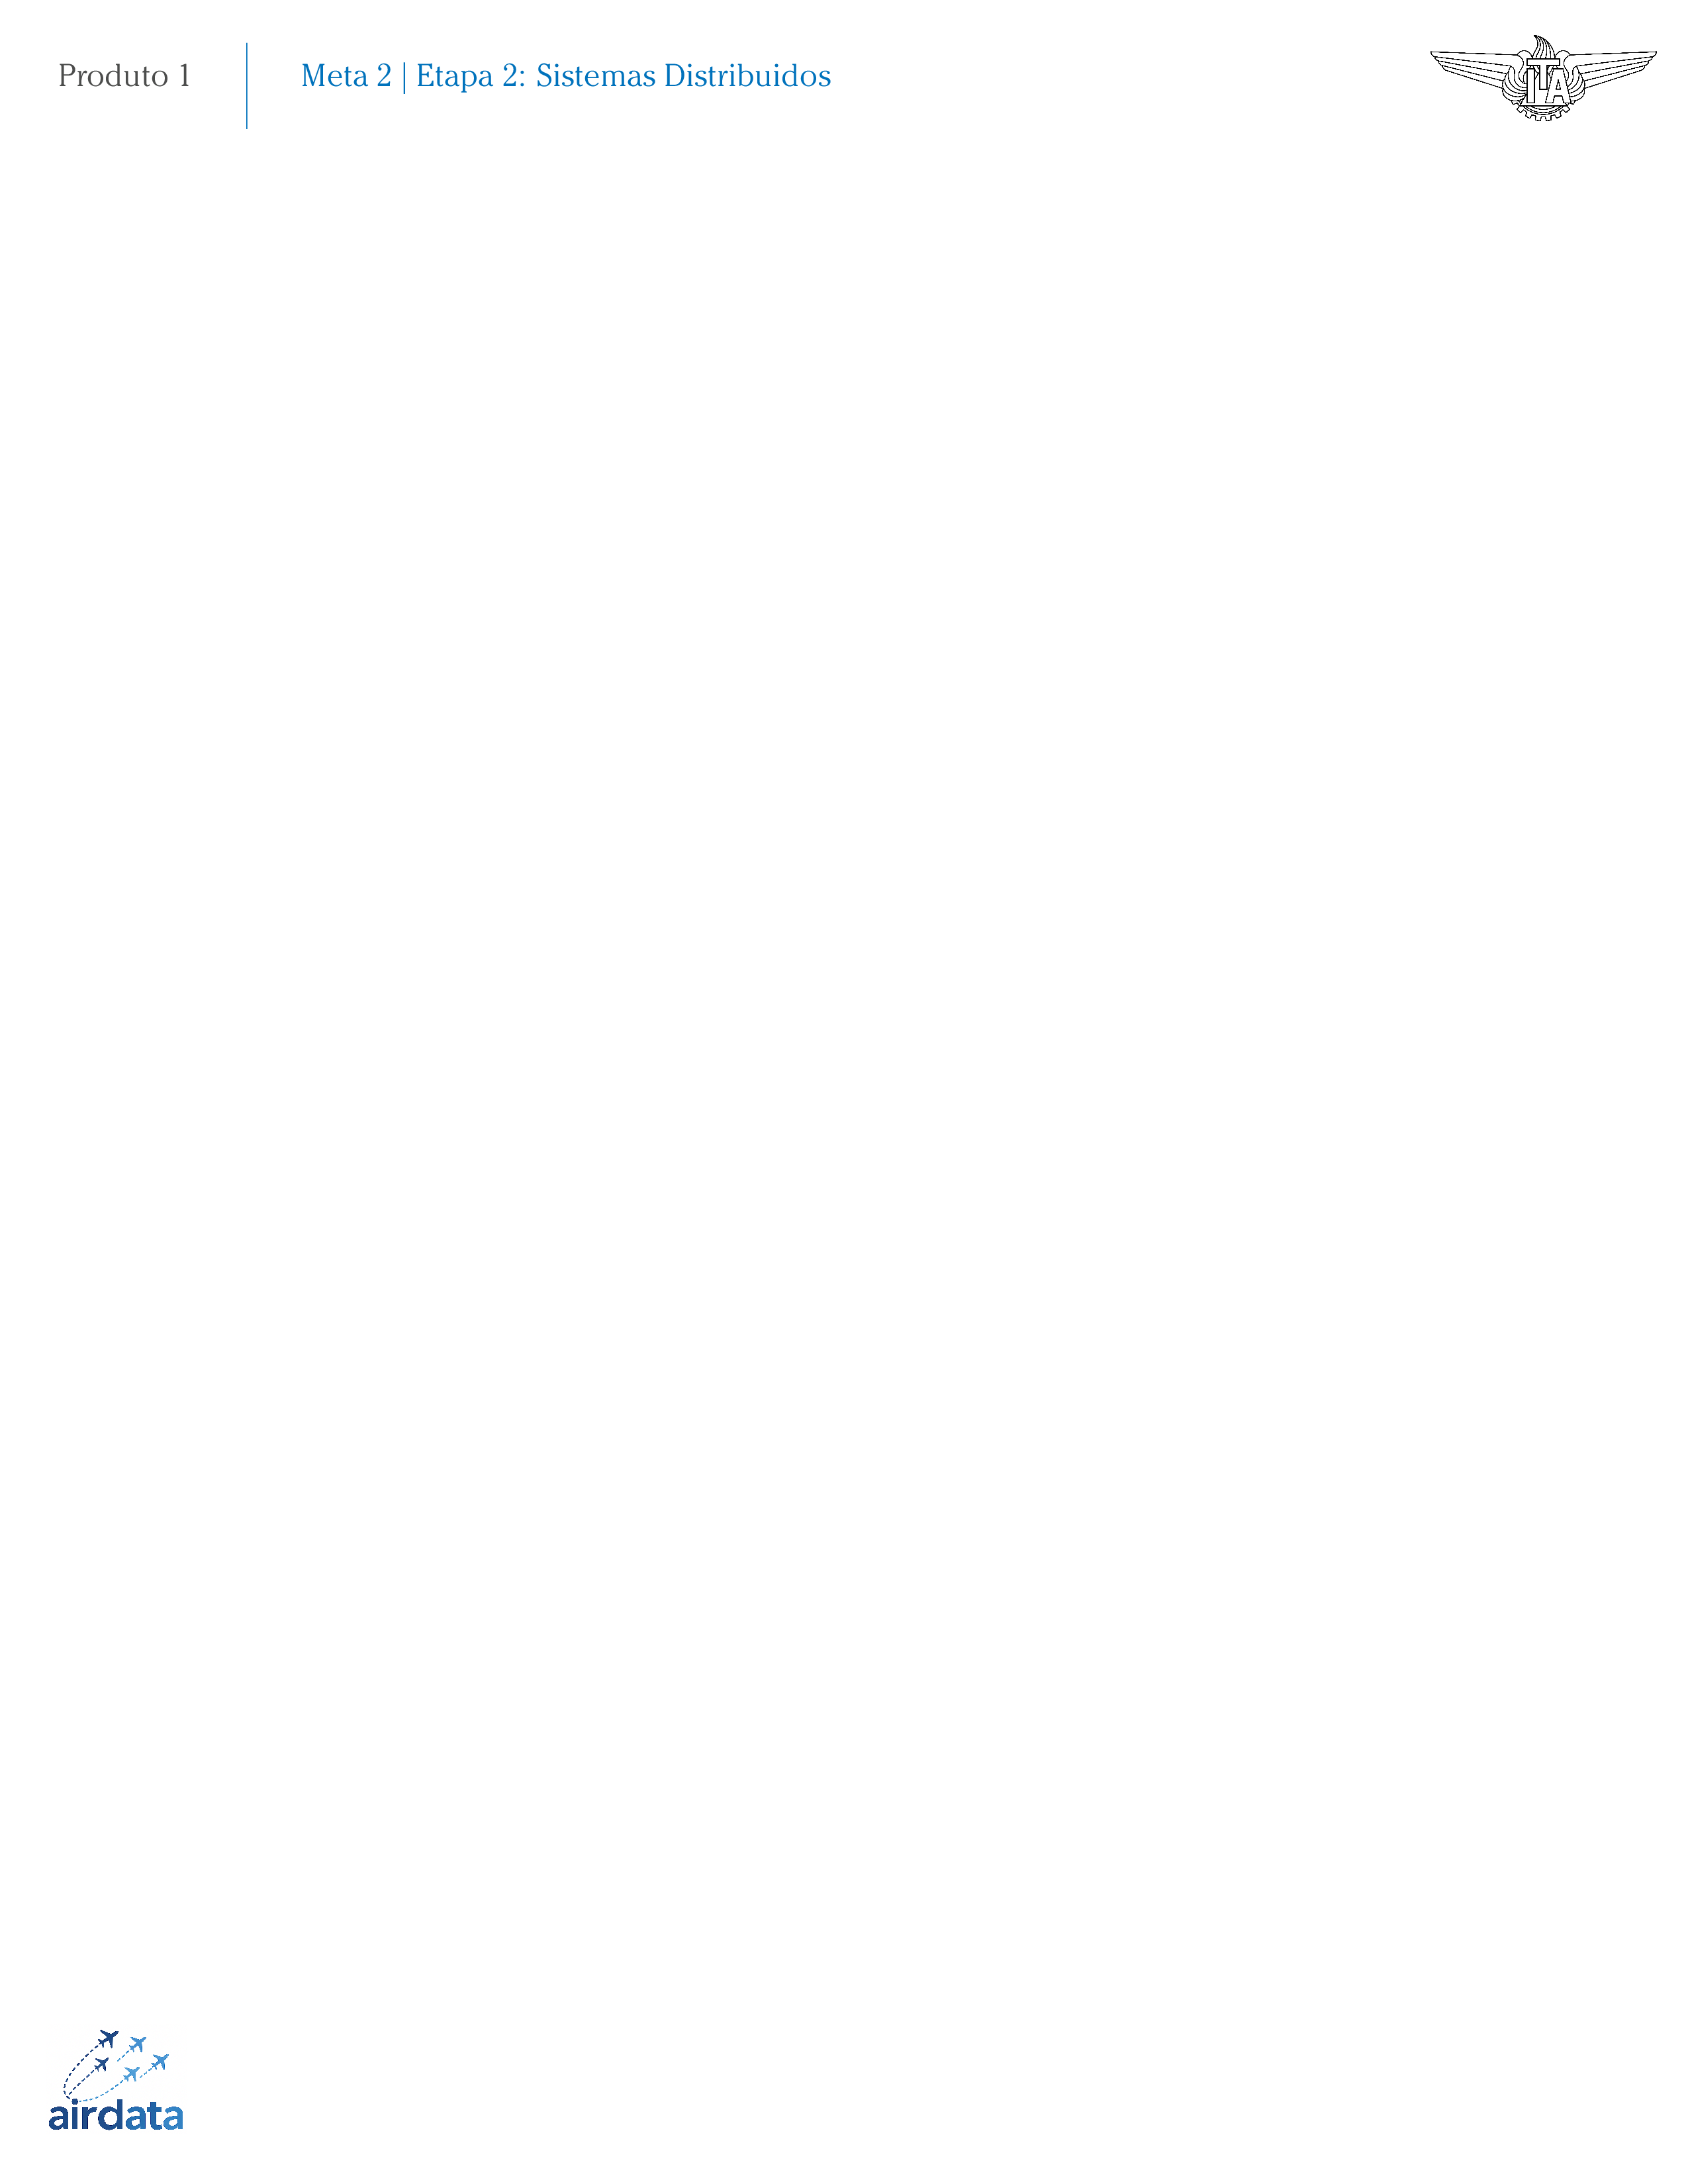
\includegraphics[width=\paperwidth,height=\paperheight]{capas/background.png}%
			\vfill
		}%
	}%
}

% Aplica a imagem de fundo em TODAS as páginas
\AddToShipoutPictureBG{\BackgroundPic}

% settings/pretextualpages.tex
% Define o background exclusivo para páginas pré-textuais

\newenvironment{pretextualblock}
{
	\ClearShipoutPictureBG
	\AddToShipoutPictureBG{
		\put(0,0){
			\parbox[b][\paperheight]{\paperwidth}{%
				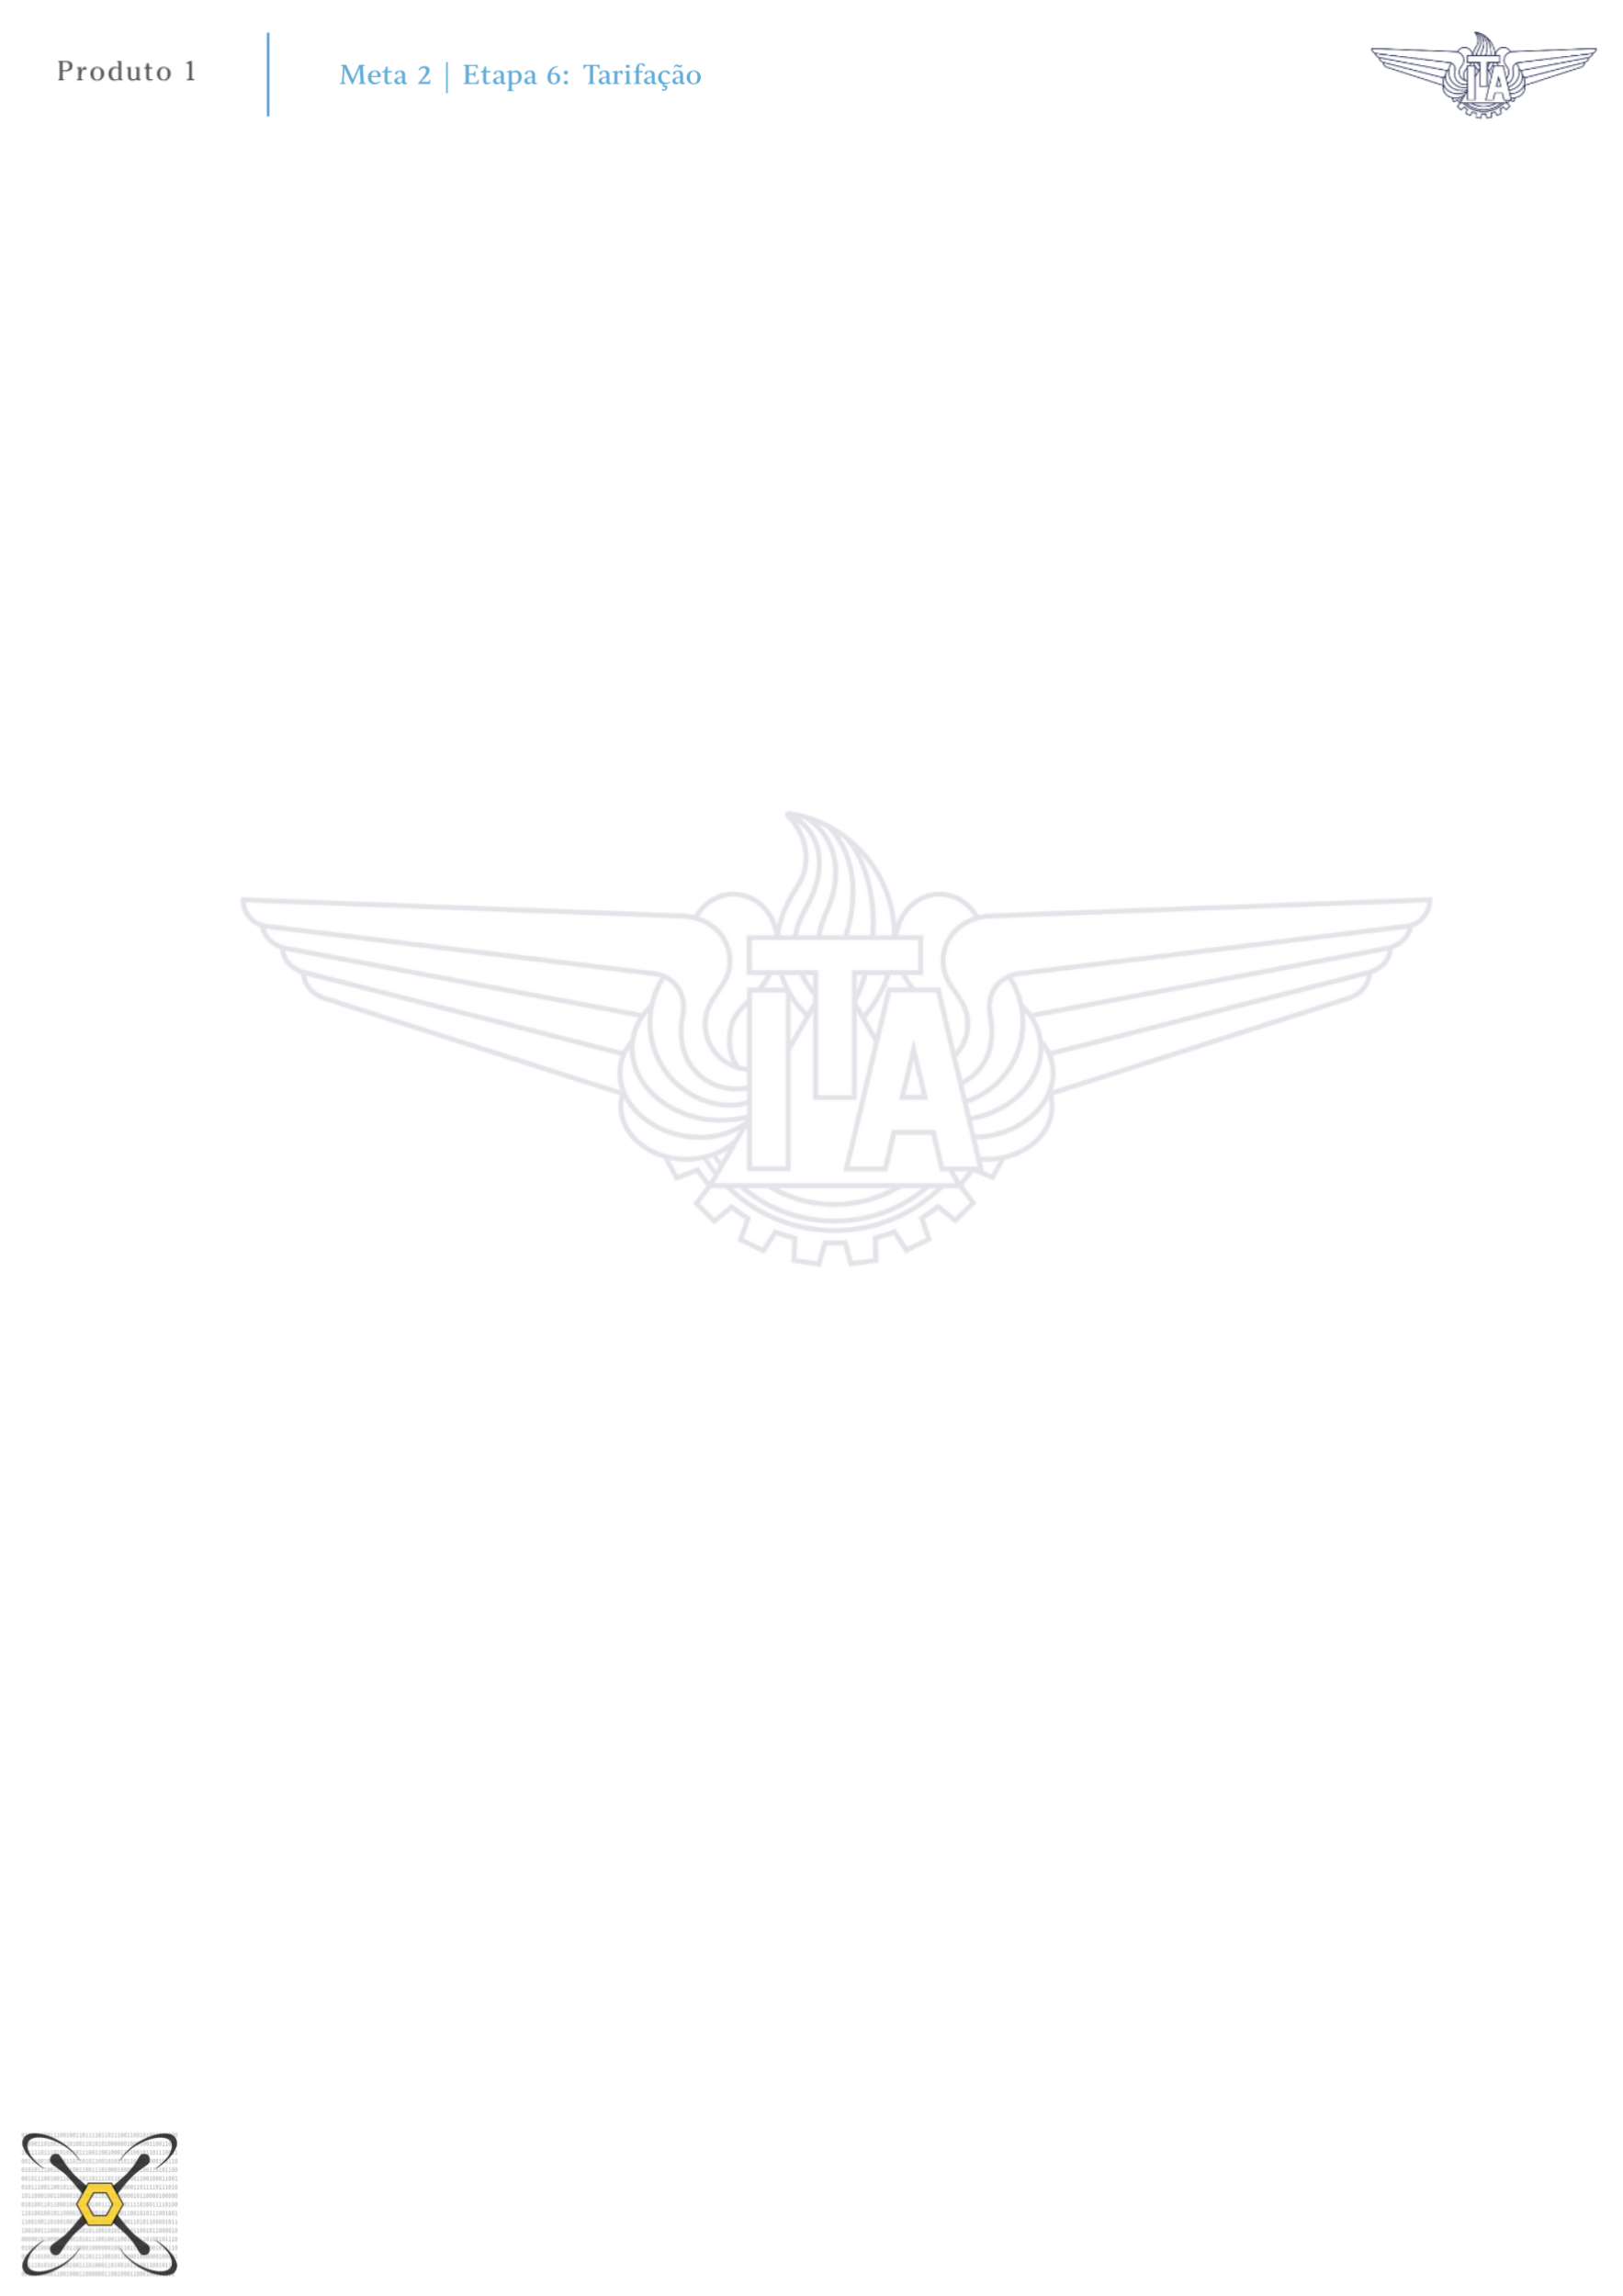
\includegraphics[width=\paperwidth,height=\paperheight]{capas/background_pretex}%
			}
		}
	}
}
{
	% settings/background.tex
% --- Imagem de fundo em todas as páginas ---

% Comando seguro para definir a imagem de fundo
\providecommand\BackgroundPic{%
	\put(0,0){%
		\parbox[b][\paperheight]{\paperwidth}{%
			\vfill
			\centering
			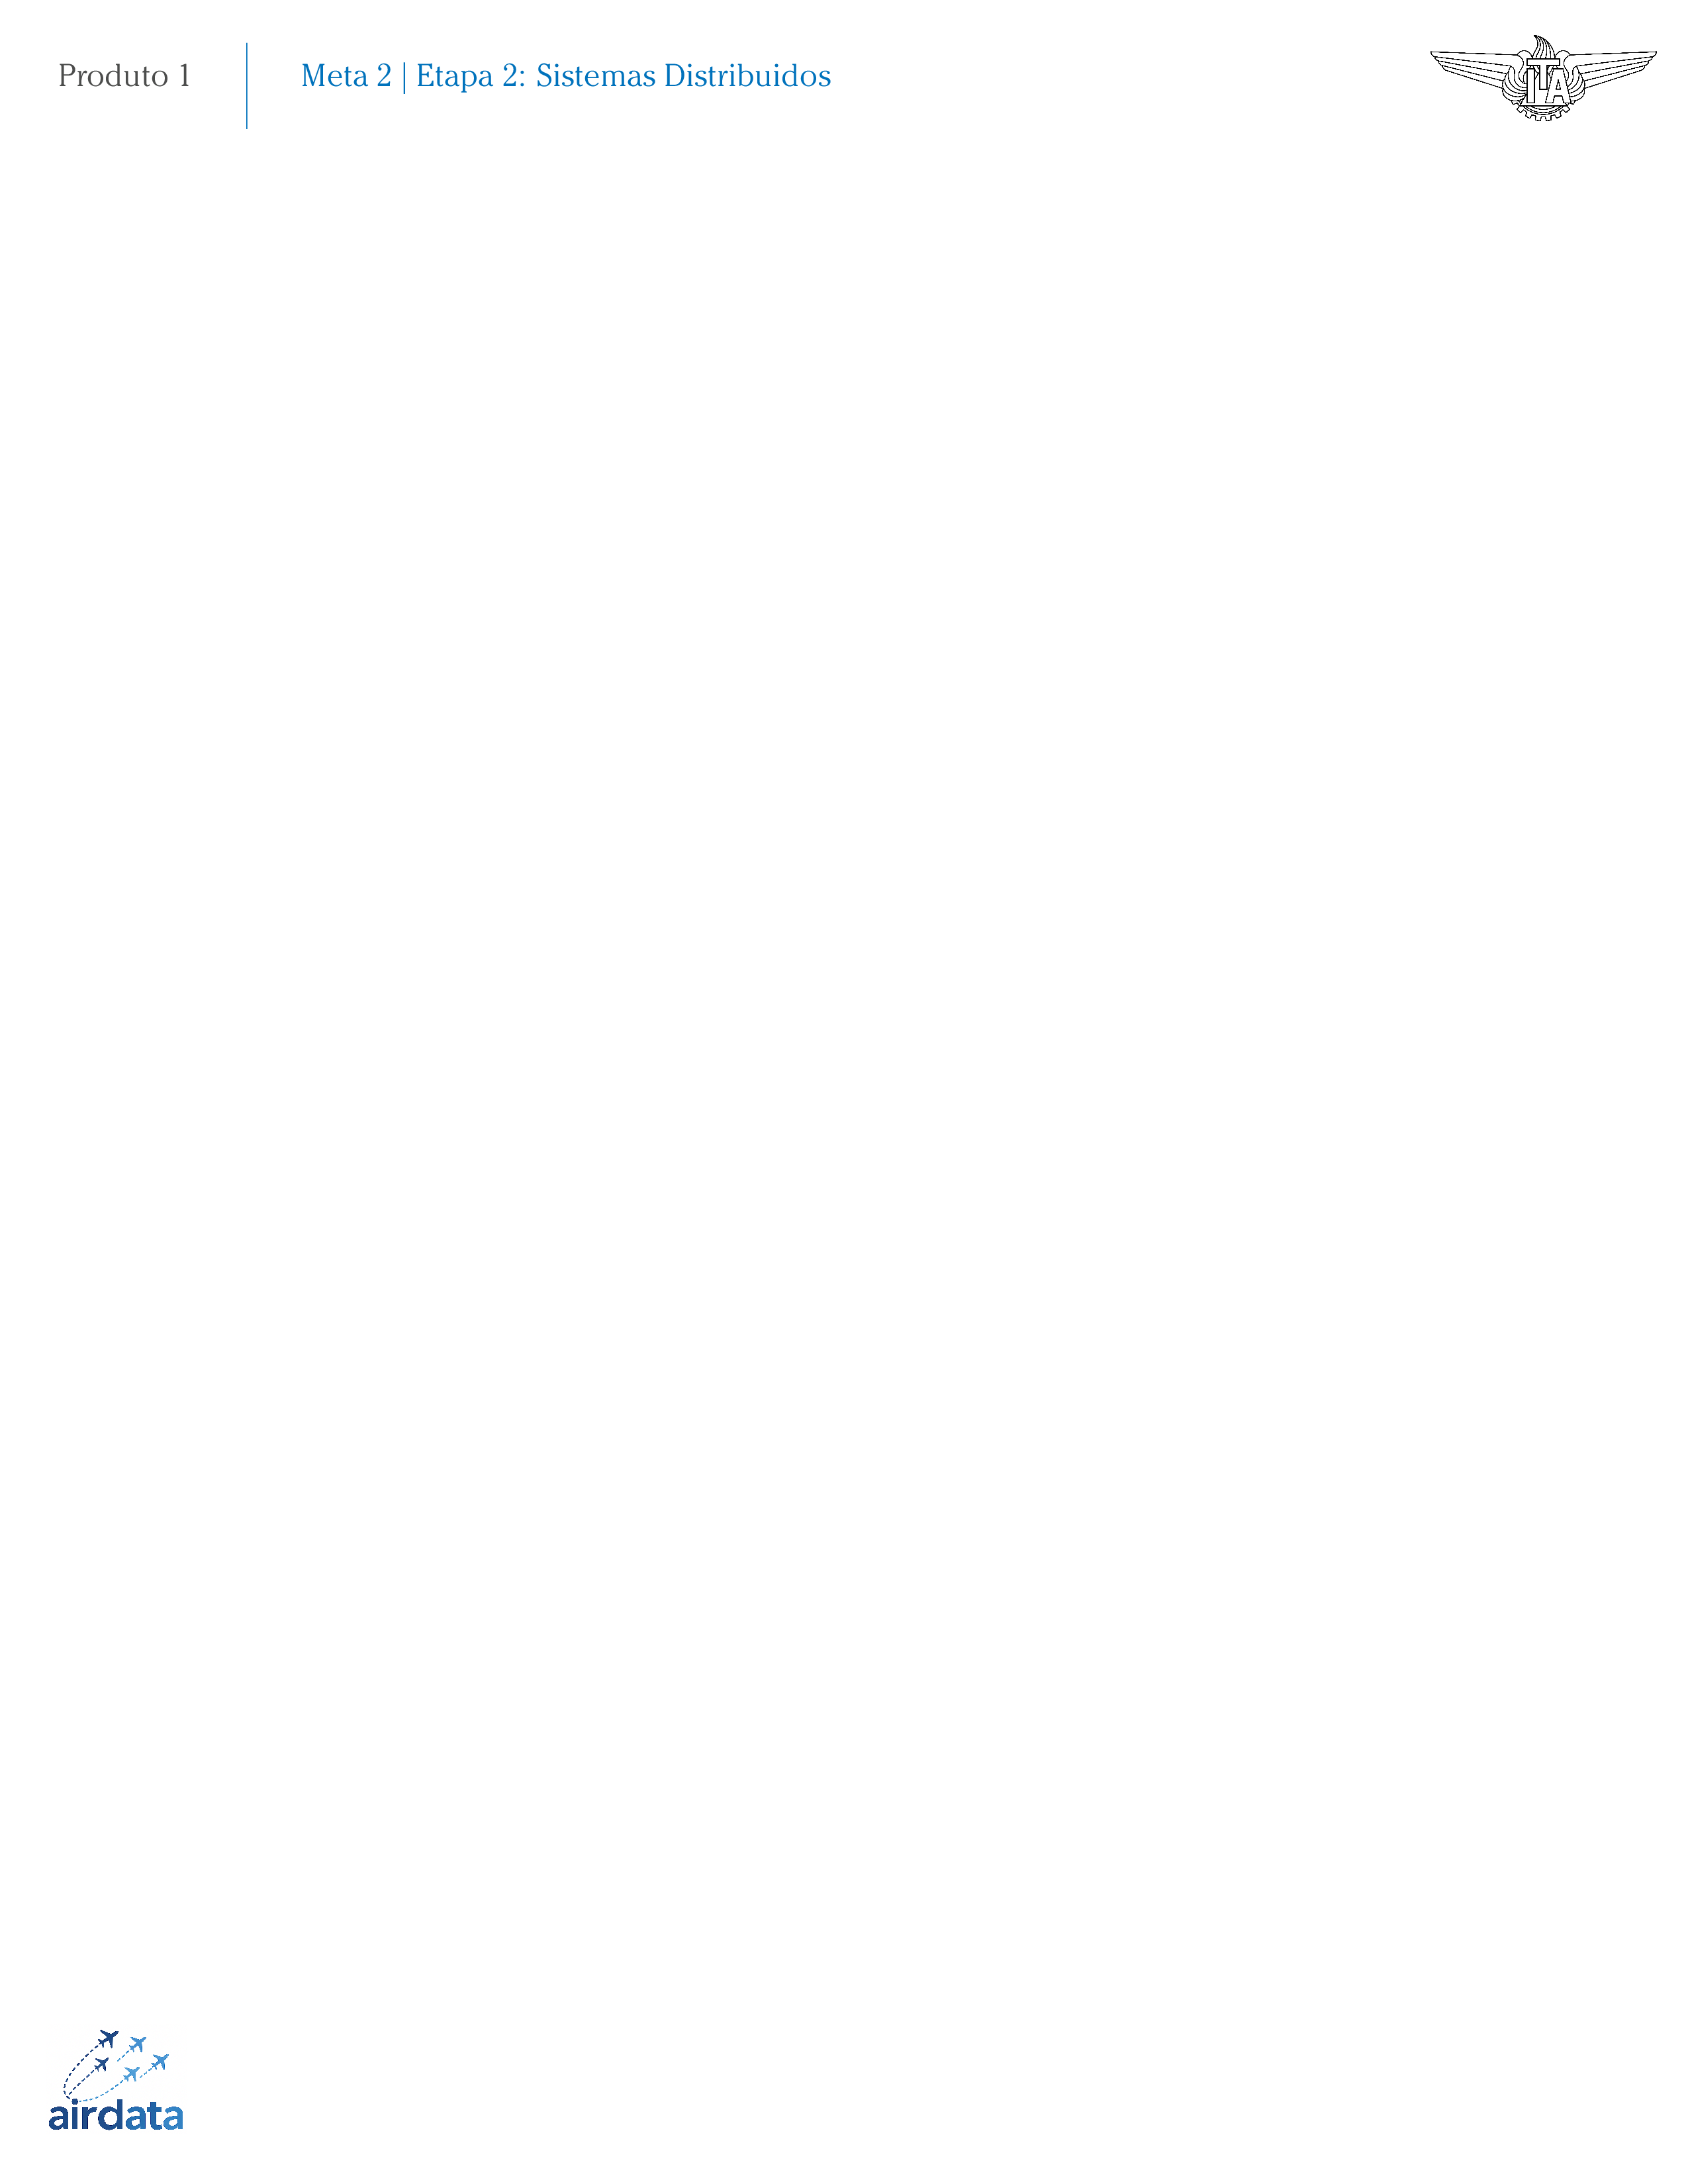
\includegraphics[width=\paperwidth,height=\paperheight]{capas/background.png}%
			\vfill
		}%
	}%
}

% Aplica a imagem de fundo em TODAS as páginas
\AddToShipoutPictureBG{\BackgroundPic}
 % Restaura o background padrão
}

\end{verbatim}

Essa ordem é proposital para garantir que os pacotes e estilos sejam carregados antes dos elementos visuais como capa e plano de fundo.

\section{Sugestão de novos capítulos}

Novos arquivos podem ser adicionados à pasta \texttt{caps/} com nomes como \texttt{cap03.tex}, \texttt{cap04.tex}, etc. A inclusão no documento é feita via:

\begin{verbatim}
\chapter{Estrutura do Template}

O template TED ITA-SAC foi organizado de forma modular, para facilitar manutenção, reuso e colaboração entre diferentes autores. A estrutura principal está organizada da seguinte forma:

\section{Visão geral}

\begin{verbatim}
	.
	|- main.tex                 % Arquivo principal (documento raiz)
	|- settings/                % Configurações gerais
	|  |- background.tex        % Marca d’água e fundo
	|  |- coverpage.tex         % Página de capa
	|  |- fonts.tex             % Fonte Cheltenham
	|  |- pretextualpages.tex  % Sumário, listas, elementos iniciais
	|  |- setabnt.tex          % Estilo de citação ABNT
	|  |- setcolor.tex         % Paleta de cores do template
	|  |- setlayout.tex        % Margens, espaçamento, cabeçalho
	|  |- settitles.tex        % Estilo de títulos e capítulos
	|  \_ usepackage.tex       % Pacotes utilizados no projeto
	|- caps/                   % Capítulos do relatório
	|  |- cap00.tex            % Introdução
	|  |- cap01.tex            % Conteúdo específico
	|  \_ etc.
	|- siglas/                 % (Opcional) Siglas, glossários
	|- refs/                   % (Opcional) Arquivos .bib
	\_ Makefile                % Automação de compilação
\end{verbatim}


\section{Função de cada componente}

\begin{itemize}
    \item \texttt{main.tex}: ponto de entrada do projeto. Controla a ordem dos elementos.
    \item \texttt{settings/}: conjunto de arquivos para configurar todos os aspectos do template.
    \item \texttt{caps/}: contém os capítulos do relatório (modularizados).
    \item \texttt{siglas/}: pasta destinada ao glossário e acrônimos, caso ativado.
    \item \texttt{refs/}: local sugerido para o arquivo de bibliografia (\texttt{.bib}).
    \item \texttt{Makefile}: automatiza as etapas de compilação (XeLaTeX + BibTeX + Glossário).
\end{itemize}

\section{Ordem de carregamento no \texttt{main.tex}}

O arquivo \texttt{main.tex} importa os componentes da seguinte forma:

\begin{verbatim}
% defs_setusepackage.tex
% --- PACOTES DO TEMPLATE AIRDATA ---


% --- Tipografia e fontes ---
\usepackage{fontspec}       % Uso de fontes OpenType com XeLaTeX

% --- Cores institucionais ---
\usepackage{xcolor}         % Suporte a cores em HTML, RGB etc.

% --- Gráficos e imagens ---
\usepackage{graphicx}       % Inclusão de imagens (.png, .pdf etc.)
\usepackage{eso-pic}        % Permite inserir elementos em todas as páginas (fundo, logos)

% --- Formatação e layout ---

\usepackage{fancyhdr}       % Cabeçalho e rodapé customizados
\usepackage{titlesec}       % Personalização de títulos (\chapter, \section etc.)

% --- Tabelas ---
\usepackage{array}
\usepackage{booktabs}
\usepackage{float}
\usepackage{tabularx}

\usepackage[acronym]{glossaries-extra}
\setabbreviationstyle[acronym]{long-short}
\makeglossaries


% Pacotes ABNT
\usepackage[alf]{abntex2cite}  % ou [num] para numérico
% settings/setabnt.tex
% --- Configurações gerais para padrão ABNT (relatórios acadêmicos) ---

% --------------------------
% Idioma
% --------------------------
\usepackage{polyglossia}
\setdefaultlanguage{portuguese}


% --------------------------
% Margens ABNT (NBR 14724)
% Esquerda e superior: 3 cm | Direita e inferior: 2 cm
% --------------------------
\usepackage[a4paper,top=3cm,bottom=2cm,left=3cm,right=2cm]{geometry}

% --------------------------
% Espaçamento entre linhas (1.5) — ABNT exige entre 1.5 e 2.0
% --------------------------
\usepackage{setspace}
\onehalfspacing

% --------------------------
% Espaçamento entre parágrafos: nenhum (ABNT)
% Recuo da primeira linha de cada parágrafo (1.25 cm recomendado)
% --------------------------

\setlength{\parindent}{0pt}   % Remove o recuo de parágrafos
\setlength{\parskip}{1em}     % Adiciona espaço entre parágrafos (opcional)

% settings/setlayout.tex
% --- Configuração de layout de página e numeração ---

\usepackage{fancyhdr}
\pagestyle{fancy}

\fancyhf{}                    % Limpa cabeçalho e rodapé
\fancyfoot[R]{\thepage}       % Número da página no canto inferior direito
\renewcommand{\headrulewidth}{0pt} % Remove linha superior
\renewcommand{\footrulewidth}{0pt} % Remove linha inferior
\setlength{\footskip}{30pt}   % Espaço do rodapé

% Aplica o mesmo layout à página de abertura dos capítulos
\fancypagestyle{plain}{%
	\fancyhf{}
	\fancyfoot[R]{\thepage}
	\renewcommand{\headrulewidth}{0pt}
	\renewcommand{\footrulewidth}{0pt}
}

% defs_fonts.tex
% --- Fontes utilizadas no template AIRDATA ---

% Define a fonte principal do documento
\setmainfont{CheltenhamITCPro-Book}[
Path = ./fonts/,
Extension = .otf,
ItalicFont = CheltenhamITCPro-BookItalic,
BoldFont = CheltenhamITCPro-Bold,
BoldItalicFont = CheltenhamITCPro-BoldItalic
]

% Define a fonte "Light" como comando \useFontLight
\newfontfamily\useFontLight{CheltenhamITCPro-Light}[
Path = ./fonts/,
Extension = .otf,
ItalicFont = CheltenhamITCPro-LightItalic
]

% Define a fonte "Ultra" como comando \useFontUltra
\newfontfamily\useFontUltra{CheltenhamITCPro-Ultra}[
Path = ./fonts/,
Extension = .otf,
ItalicFont = CheltenhamITCPro-UltraItalic
]


\providecommand{\useFontLight}{}
\providecommand{\useFontUltra}{}

% settings/setcolor.tex
% --- Definições de cores do projeto AIRDATA ---

% Importante: não utilize o comando \usepackage{xcolor} aqui.
% Esse pacote já está carregado no arquivo settings/usepackage.tex.

% Cor azul institucional AIRDATA
\definecolor{airdataBlue}{HTML}{2f84c6}

% ========================================
% PALETA DE CORES - METAS E ETAPAS
% ========================================

% Cores de Coordenação
\definecolor{coordMeta1}{HTML}{272a6a}
\definecolor{coordMeta2}{HTML}{388fcd}

% --- META 1 ---
\definecolor{meta1etapa1}{HTML}{283880}
\definecolor{meta1etapa2}{HTML}{204196}
\definecolor{meta1etapa3}{HTML}{2451a4}
\definecolor{meta1etapa4}{HTML}{2b61ae}
\definecolor{meta1etapa5}{HTML}{2d72ba}
\definecolor{meta1etapa6}{HTML}{2f84c6}

% --- META 2 ---
\definecolor{meta2etapa1}{HTML}{388fcd}
\definecolor{meta2etapa2}{HTML}{6597ca}
\definecolor{meta2etapa3}{HTML}{6392bd}
\definecolor{meta2etapa4}{HTML}{618eb1}
\definecolor{meta2etapa5}{HTML}{5e89a7}
\definecolor{meta2etapa6}{HTML}{5c859c}
\definecolor{meta2etapa7}{HTML}{4d7d94}
\definecolor{meta2etapa8}{HTML}{3f738b}
\definecolor{meta2etapa9}{HTML}{306983}
\definecolor{meta2etapa10}{HTML}{215f7b}

% ========================================
% CORES ESPECIAIS PARA CAPAS
% ========================================

% Cor creme para fundo de capa (conforme feedback ChatGPT)
\definecolor{creamBg}{RGB}{250,245,225}

% ========================================
% COR PRINCIPAL DO PROJETO
% ========================================

% Cor principal do projeto (Meta 2 Etapa 6 por padrão)
% Esta cor é usada para destacar o projeto atual na paleta
\definecolor{projectMainColor}{named}{meta2etapa6}

% settings/settitles.tex
% --- Estilo e formatação dos títulos do template AIRDATA ---

\RequirePackage{titlesec}

% Mostra a numeração até subsubsection
\setcounter{secnumdepth}{3}

% -------------------------------
% CAPÍTULO (CHAPTER) — 16 pt, azul, normal
% -------------------------------
\titleformat{\chapter}[hang]
{\color{airdataBlue}\normalfont\fontsize{16}{20}\selectfont}
{\thechapter}{1em}{}

% -------------------------------
% SEÇÃO (SECTION) — 14 pt, azul, itálico
% -------------------------------
\titleformat{\section}
{\color{airdataBlue}\normalfont\fontsize{14}{18}\selectfont}
{\thesection}{1em}{}

% -------------------------------
% SUBSEÇÃO (SUBSECTION) — 14 pt, azul, itálico
% -------------------------------
\titleformat{\subsection}
{\color{airdataBlue}\normalfont\itshape\fontsize{14}{17}\selectfont}
{\thesubsection}{1em}{}

% -------------------------------
% SUBSUBSEÇÃO (SUBSUBSECTION) — 12 pt, azul, itálico
% -------------------------------
\titleformat{\subsubsection}
{\color{airdataBlue}\normalfont\itshape\fontsize{12}{14}\selectfont}
{\thesubsubsection}{1em}{}

% -------------------------------
% Espaçamento vertical entre título e texto
% -------------------------------
\titlespacing*{\chapter}      {0pt}{20pt plus 2pt}{10pt plus 2pt}
\titlespacing*{\section}      {0pt}{16pt plus 2pt}{8pt plus 2pt}
\titlespacing*{\subsection}   {0pt}{14pt plus 2pt}{6pt plus 2pt}
\titlespacing*{\subsubsection}{0pt}{12pt plus 2pt}{4pt plus 2pt}

% settings/coverpage.tex
% --- Capa com imagem de fundo ocupando toda a página ---

\newcommand\makecover{
	\ClearShipoutPictureBG  % remove o background institucional temporariamente
	\AddToShipoutPicture*{
		\put(0,0){
			
\includegraphics[width=\paperwidth,height=\paperheight]{capas/cover.png}
		}
	}
	\begin{titlepage}
		\null  % necessário para forçar a renderização da imagem
		\thispagestyle{empty}
		\newpage
	\end{titlepage}
	\ClearShipoutPictureBG  % limpa a capa para evitar efeito nas próximas páginas
	\AddToShipoutPictureBG{\BackgroundPic}  % restaura o background institucional
}

% settings/background.tex
% --- Imagem de fundo em todas as páginas ---

% Comando seguro para definir a imagem de fundo
\providecommand\BackgroundPic{%
	\put(0,0){%
		\parbox[b][\paperheight]{\paperwidth}{%
			\vfill
			\centering
			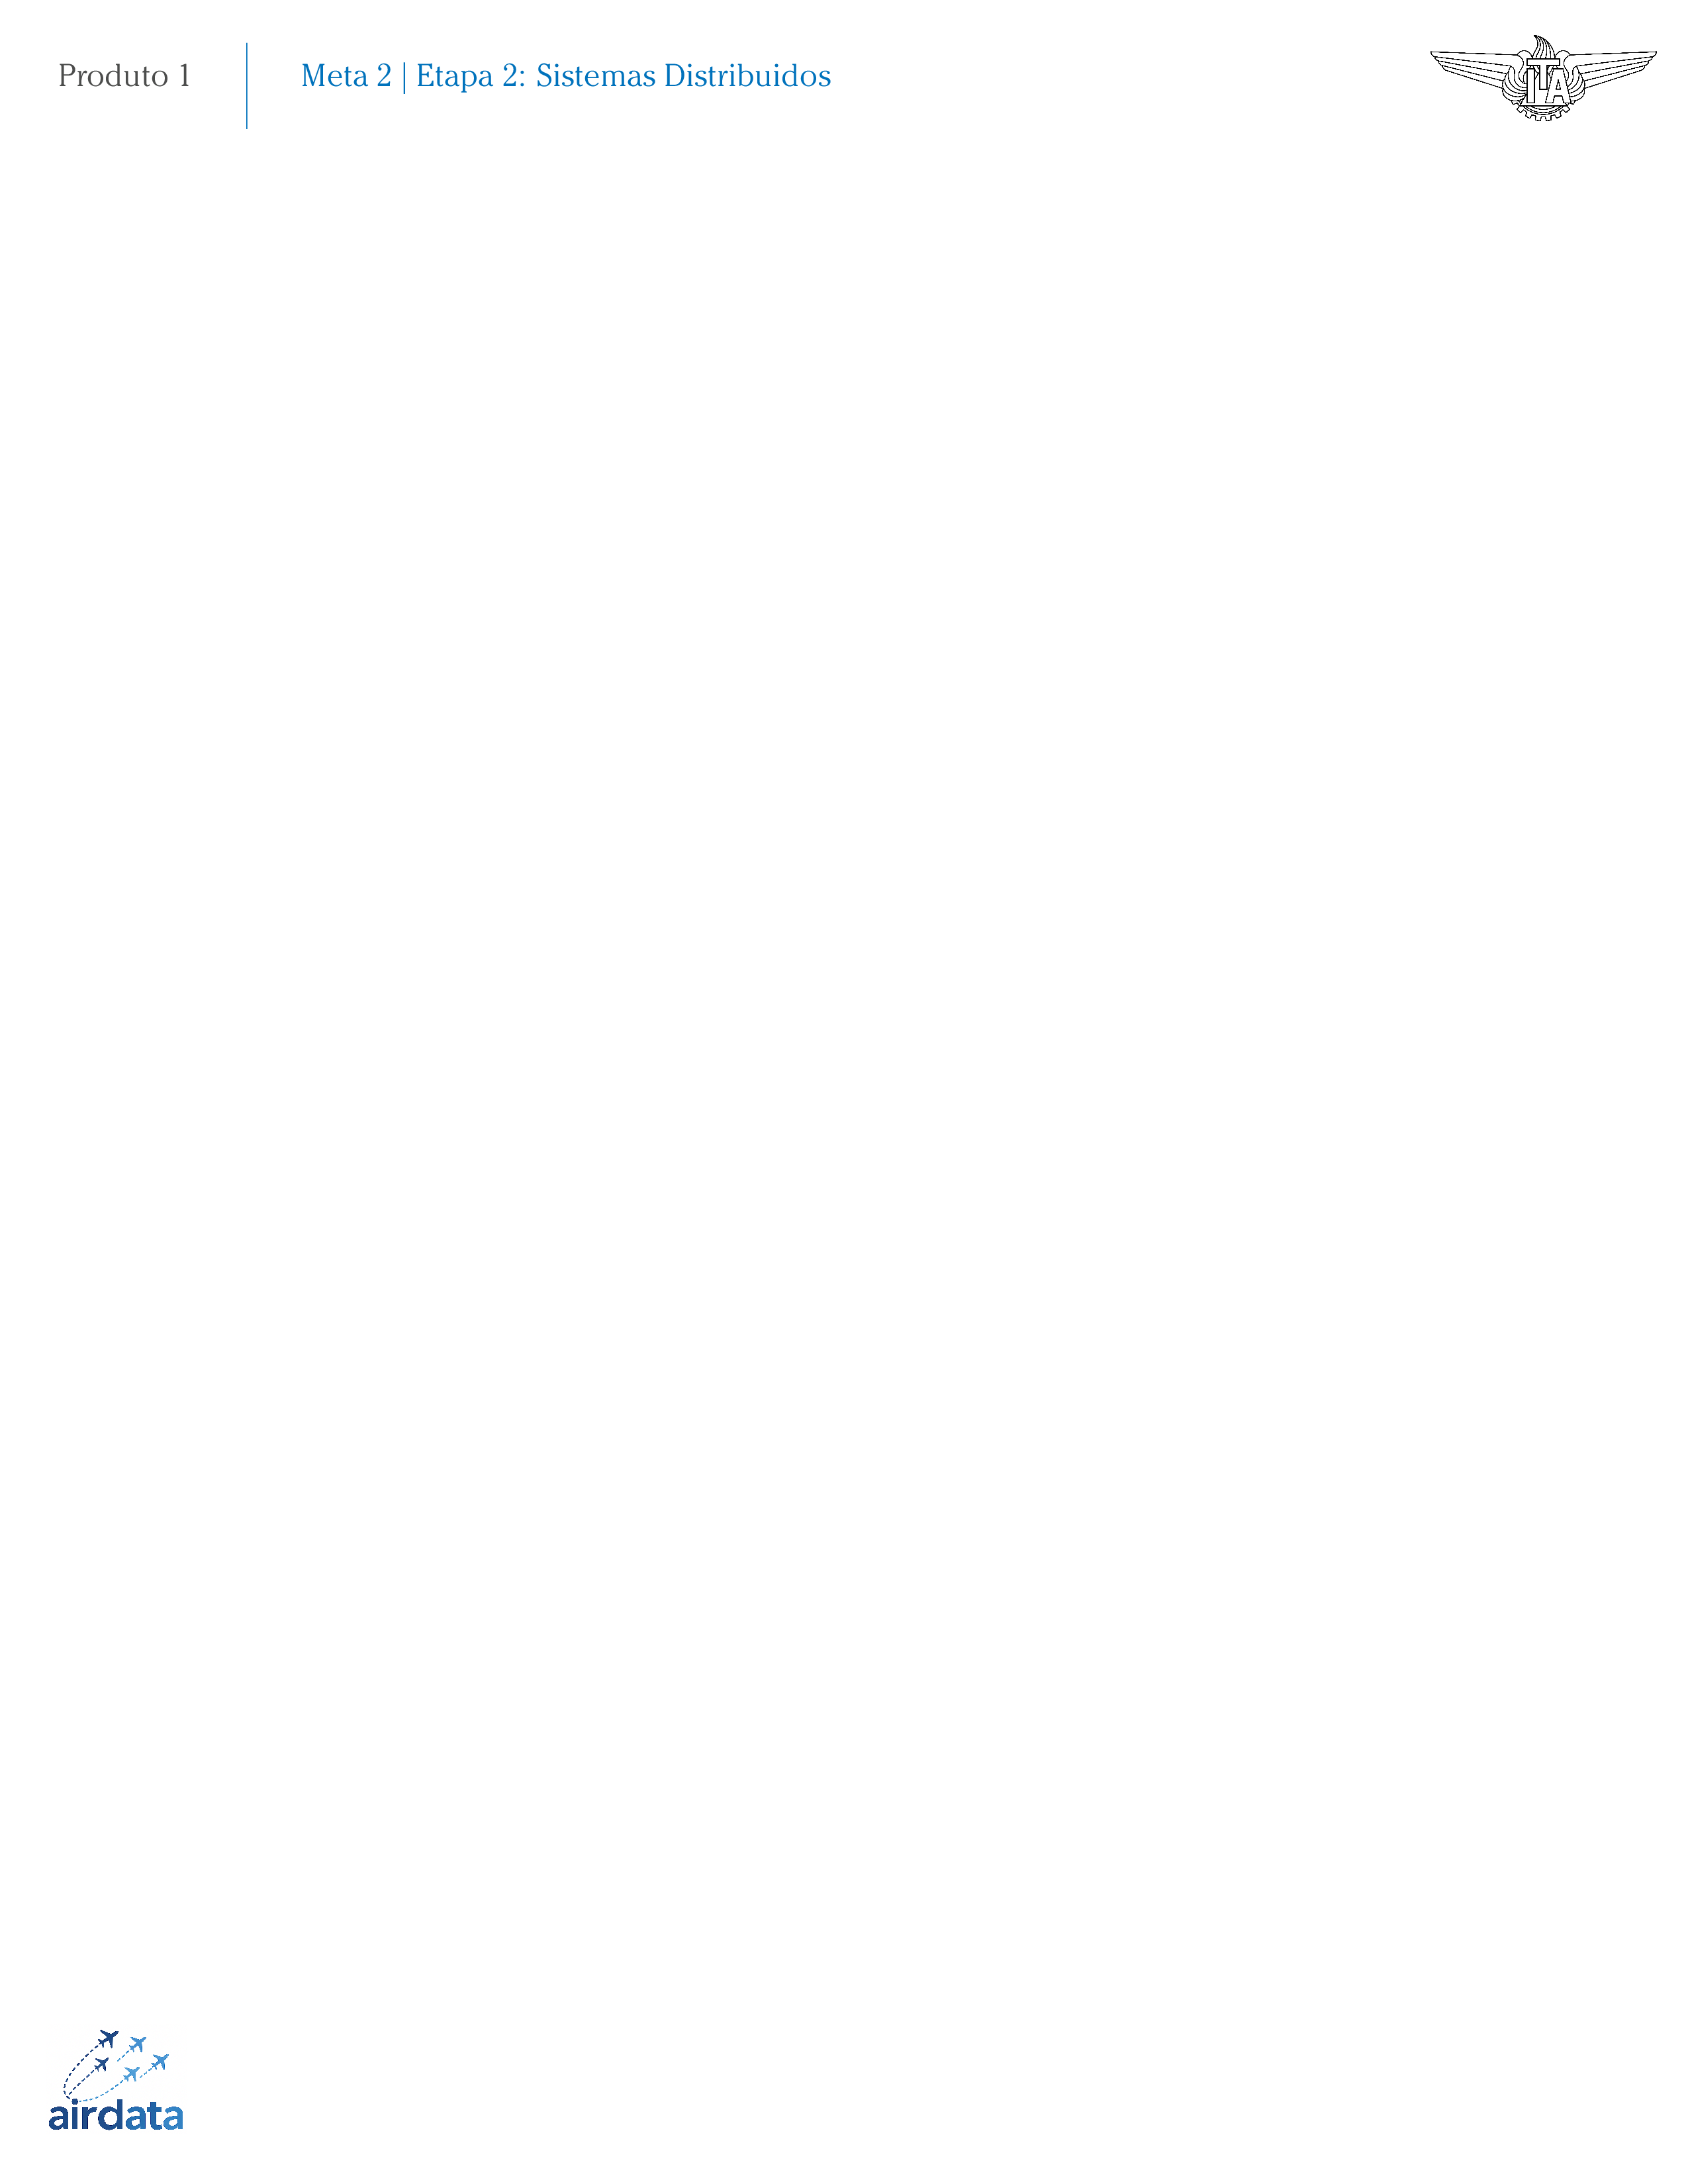
\includegraphics[width=\paperwidth,height=\paperheight]{capas/background.png}%
			\vfill
		}%
	}%
}

% Aplica a imagem de fundo em TODAS as páginas
\AddToShipoutPictureBG{\BackgroundPic}

% settings/pretextualpages.tex
% Define o background exclusivo para páginas pré-textuais

\newenvironment{pretextualblock}
{
	\ClearShipoutPictureBG
	\AddToShipoutPictureBG{
		\put(0,0){
			\parbox[b][\paperheight]{\paperwidth}{%
				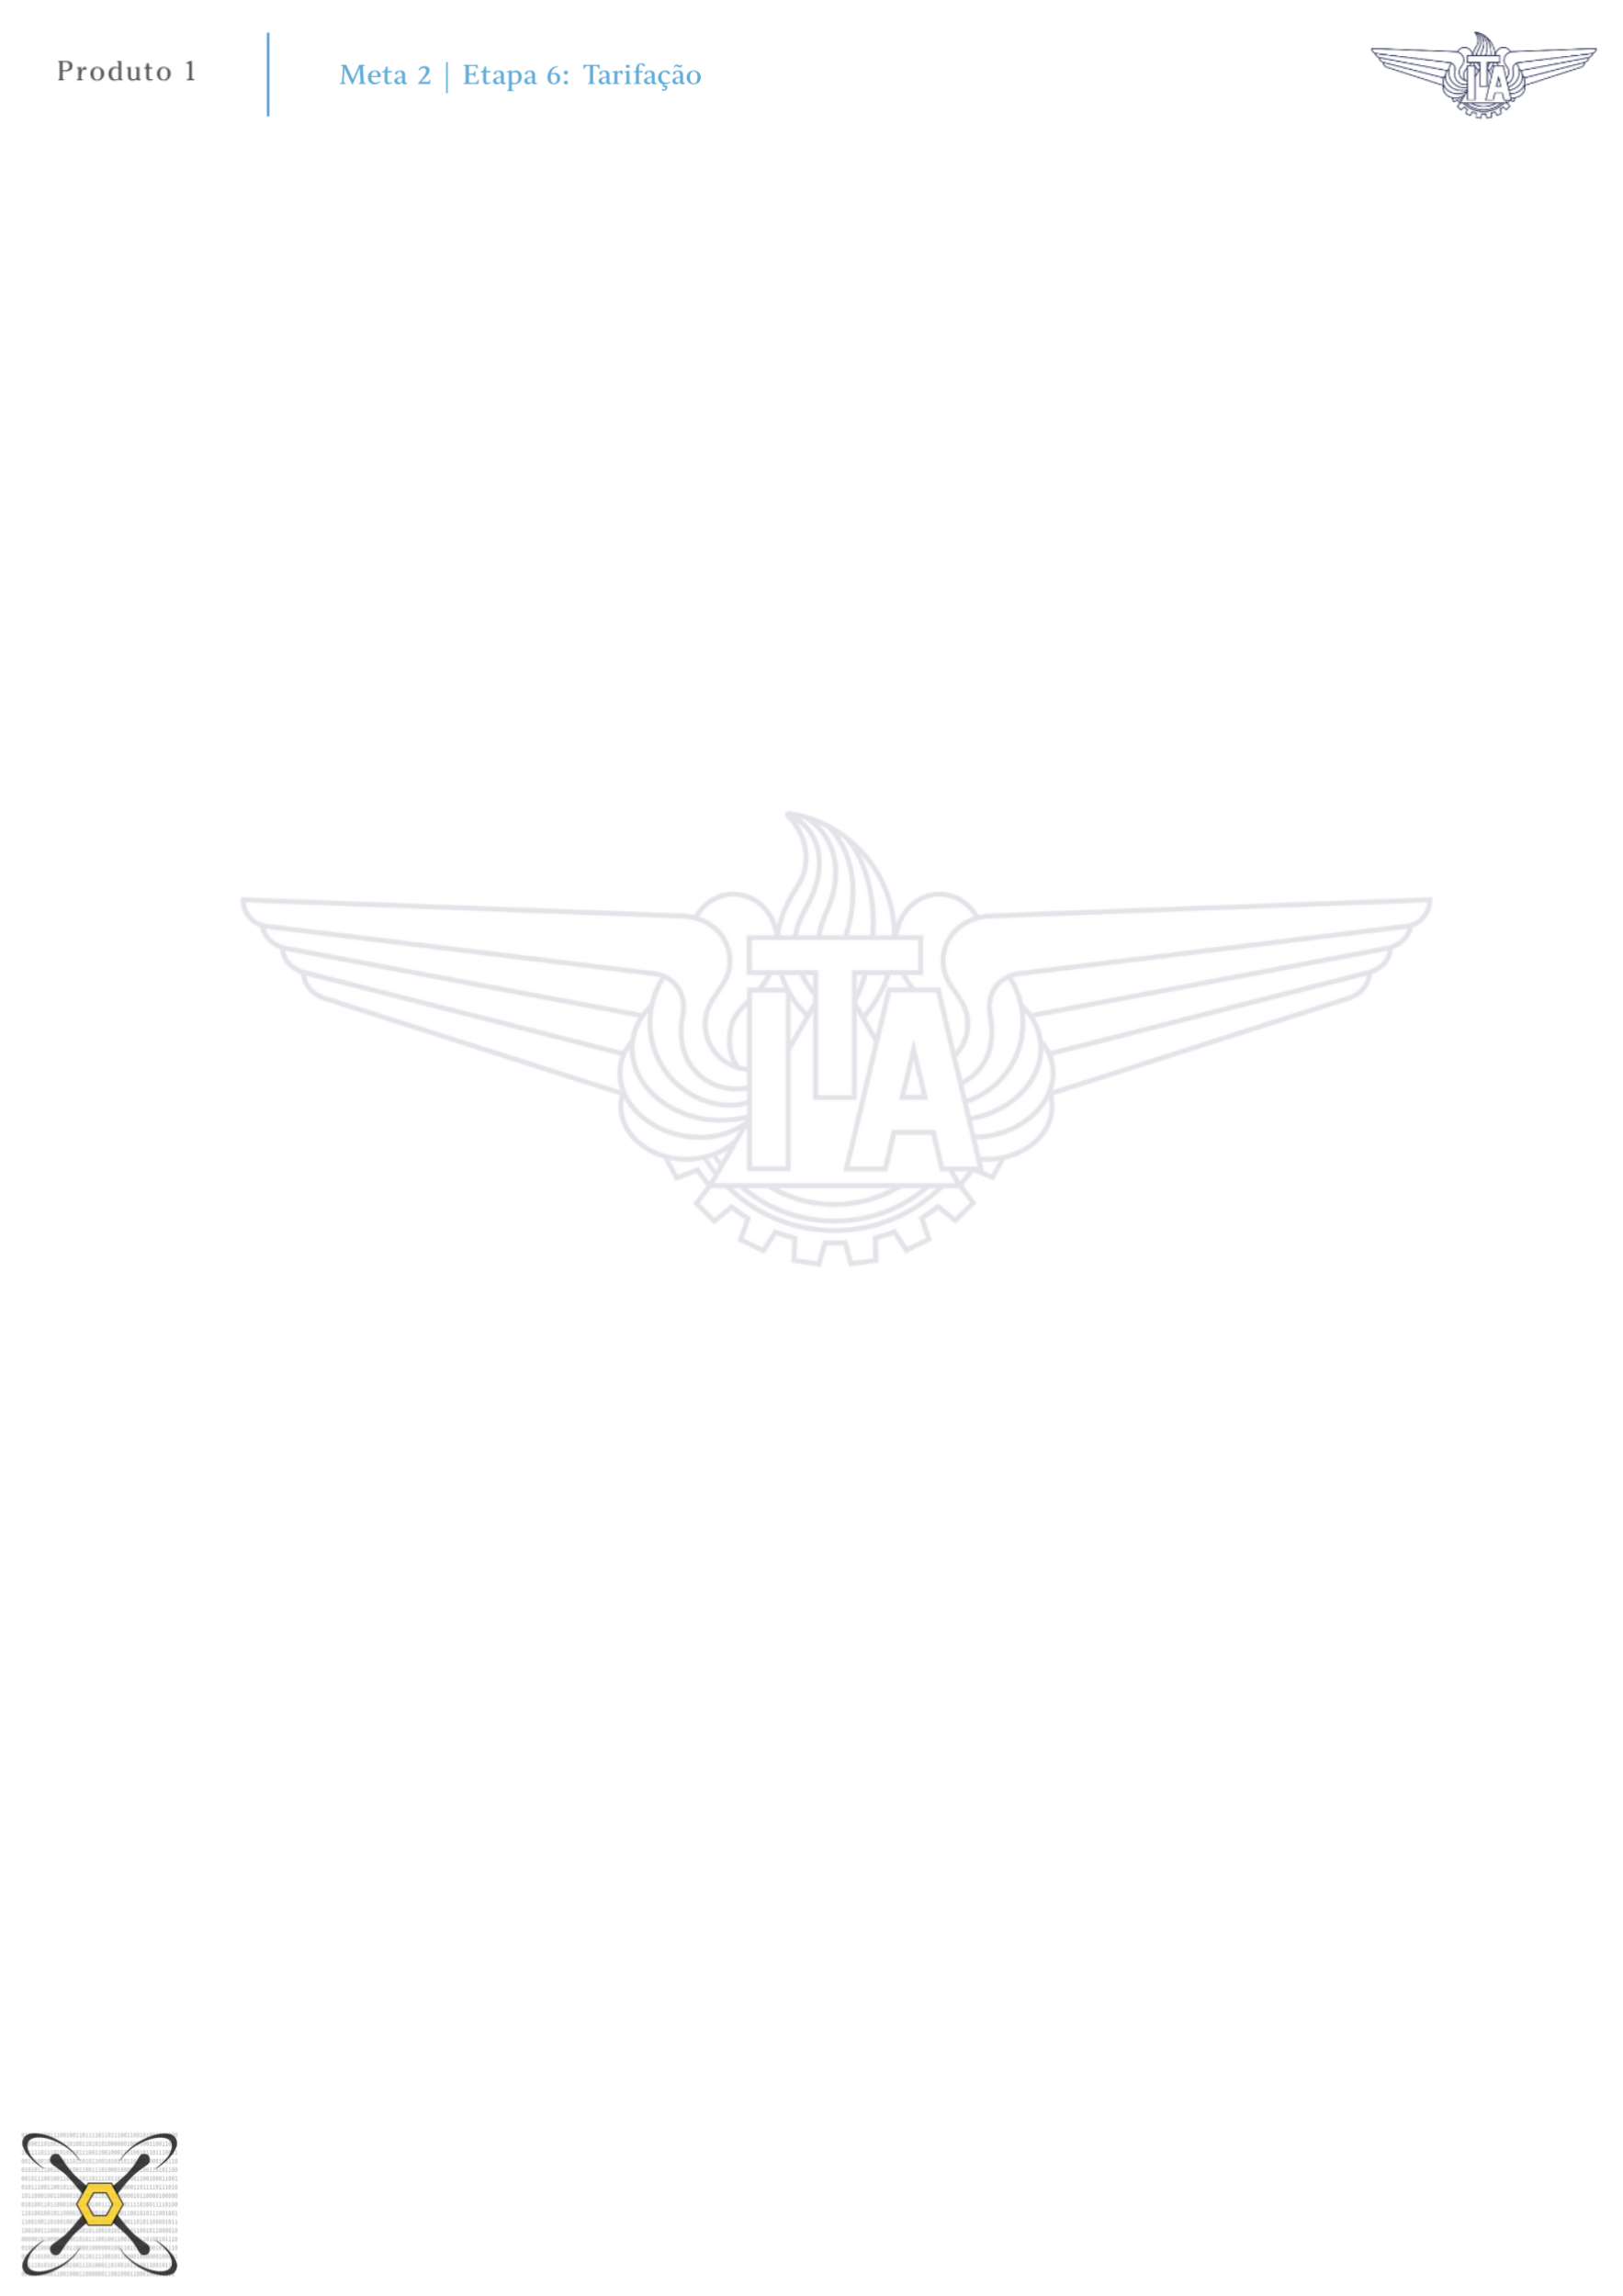
\includegraphics[width=\paperwidth,height=\paperheight]{capas/background_pretex}%
			}
		}
	}
}
{
	% settings/background.tex
% --- Imagem de fundo em todas as páginas ---

% Comando seguro para definir a imagem de fundo
\providecommand\BackgroundPic{%
	\put(0,0){%
		\parbox[b][\paperheight]{\paperwidth}{%
			\vfill
			\centering
			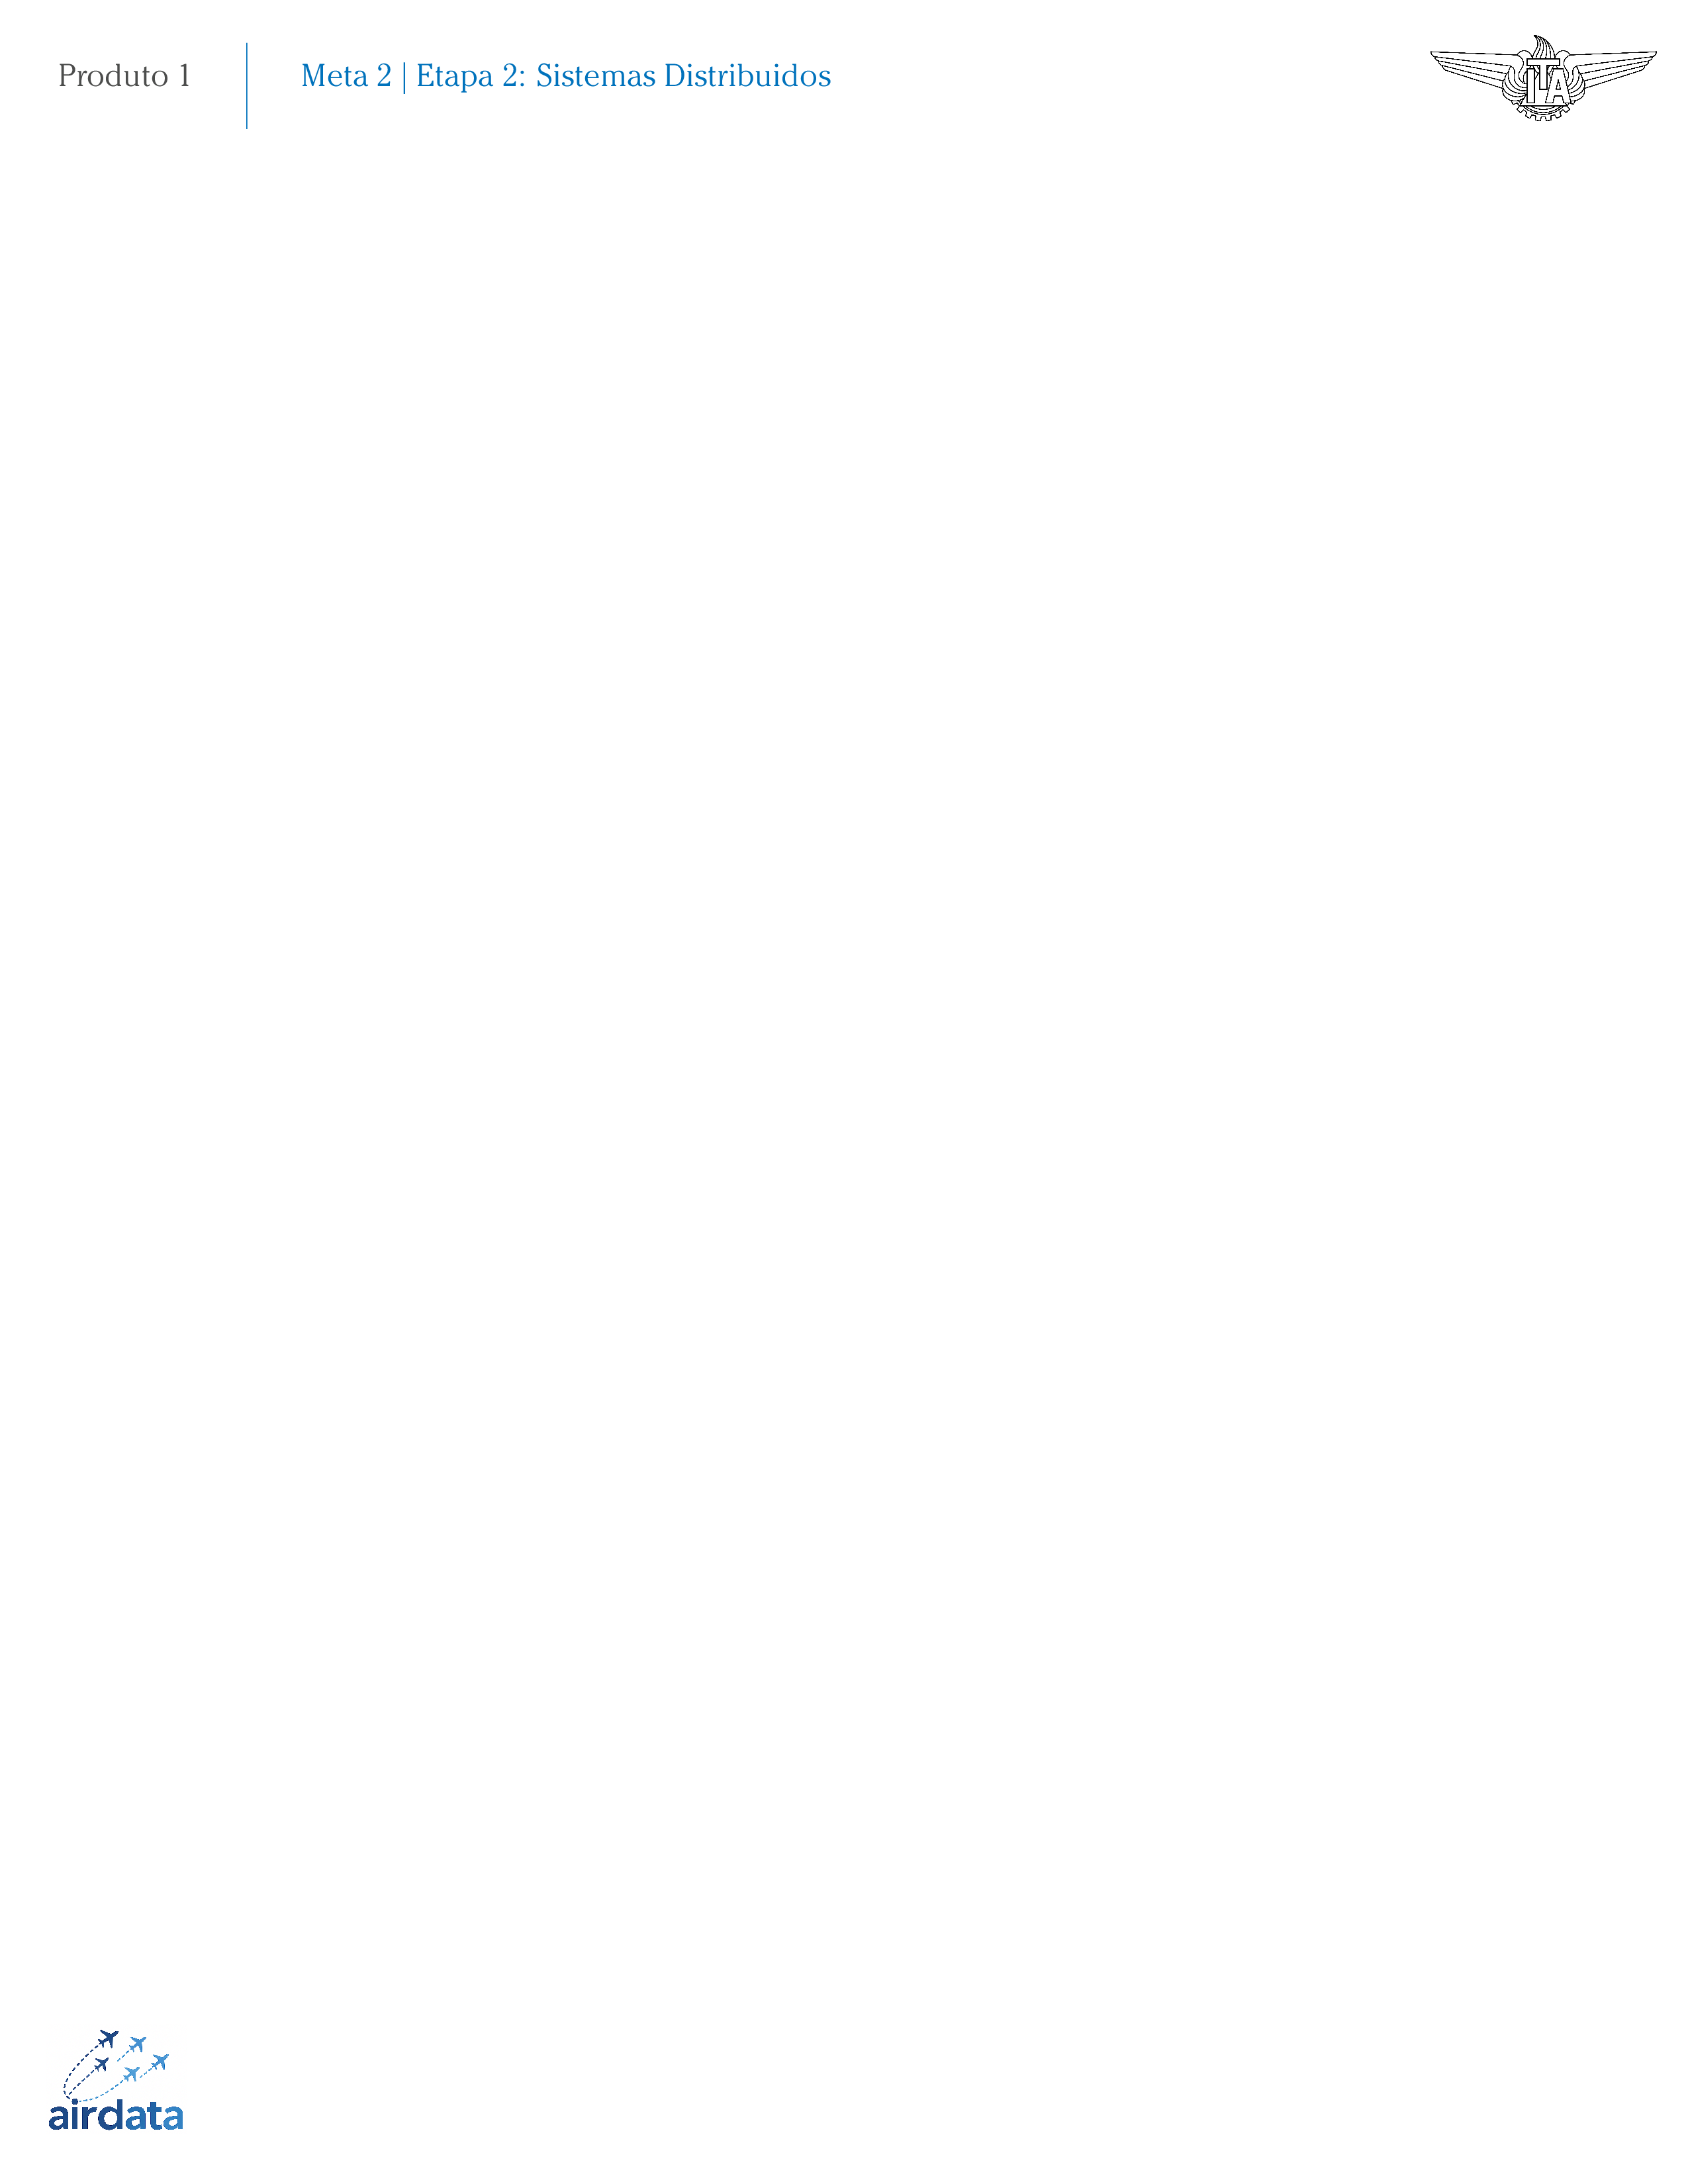
\includegraphics[width=\paperwidth,height=\paperheight]{capas/background.png}%
			\vfill
		}%
	}%
}

% Aplica a imagem de fundo em TODAS as páginas
\AddToShipoutPictureBG{\BackgroundPic}
 % Restaura o background padrão
}

\end{verbatim}

Essa ordem é proposital para garantir que os pacotes e estilos sejam carregados antes dos elementos visuais como capa e plano de fundo.

\section{Sugestão de novos capítulos}

Novos arquivos podem ser adicionados à pasta \texttt{caps/} com nomes como \texttt{cap03.tex}, \texttt{cap04.tex}, etc. A inclusão no documento é feita via:

\begin{verbatim}
\chapter{Estrutura do Template}

O template TED ITA-SAC foi organizado de forma modular, para facilitar manutenção, reuso e colaboração entre diferentes autores. A estrutura principal está organizada da seguinte forma:

\section{Visão geral}

\begin{verbatim}
	.
	|- main.tex                 % Arquivo principal (documento raiz)
	|- settings/                % Configurações gerais
	|  |- background.tex        % Marca d’água e fundo
	|  |- coverpage.tex         % Página de capa
	|  |- fonts.tex             % Fonte Cheltenham
	|  |- pretextualpages.tex  % Sumário, listas, elementos iniciais
	|  |- setabnt.tex          % Estilo de citação ABNT
	|  |- setcolor.tex         % Paleta de cores do template
	|  |- setlayout.tex        % Margens, espaçamento, cabeçalho
	|  |- settitles.tex        % Estilo de títulos e capítulos
	|  \_ usepackage.tex       % Pacotes utilizados no projeto
	|- caps/                   % Capítulos do relatório
	|  |- cap00.tex            % Introdução
	|  |- cap01.tex            % Conteúdo específico
	|  \_ etc.
	|- siglas/                 % (Opcional) Siglas, glossários
	|- refs/                   % (Opcional) Arquivos .bib
	\_ Makefile                % Automação de compilação
\end{verbatim}


\section{Função de cada componente}

\begin{itemize}
    \item \texttt{main.tex}: ponto de entrada do projeto. Controla a ordem dos elementos.
    \item \texttt{settings/}: conjunto de arquivos para configurar todos os aspectos do template.
    \item \texttt{caps/}: contém os capítulos do relatório (modularizados).
    \item \texttt{siglas/}: pasta destinada ao glossário e acrônimos, caso ativado.
    \item \texttt{refs/}: local sugerido para o arquivo de bibliografia (\texttt{.bib}).
    \item \texttt{Makefile}: automatiza as etapas de compilação (XeLaTeX + BibTeX + Glossário).
\end{itemize}

\section{Ordem de carregamento no \texttt{main.tex}}

O arquivo \texttt{main.tex} importa os componentes da seguinte forma:

\begin{verbatim}
% defs_setusepackage.tex
% --- PACOTES DO TEMPLATE AIRDATA ---


% --- Tipografia e fontes ---
\usepackage{fontspec}       % Uso de fontes OpenType com XeLaTeX

% --- Cores institucionais ---
\usepackage{xcolor}         % Suporte a cores em HTML, RGB etc.

% --- Gráficos e imagens ---
\usepackage{graphicx}       % Inclusão de imagens (.png, .pdf etc.)
\usepackage{eso-pic}        % Permite inserir elementos em todas as páginas (fundo, logos)

% --- Formatação e layout ---

\usepackage{fancyhdr}       % Cabeçalho e rodapé customizados
\usepackage{titlesec}       % Personalização de títulos (\chapter, \section etc.)

% --- Tabelas ---
\usepackage{array}
\usepackage{booktabs}
\usepackage{float}
\usepackage{tabularx}

\usepackage[acronym]{glossaries-extra}
\setabbreviationstyle[acronym]{long-short}
\makeglossaries


% Pacotes ABNT
\usepackage[alf]{abntex2cite}  % ou [num] para numérico
% settings/setabnt.tex
% --- Configurações gerais para padrão ABNT (relatórios acadêmicos) ---

% --------------------------
% Idioma
% --------------------------
\usepackage{polyglossia}
\setdefaultlanguage{portuguese}


% --------------------------
% Margens ABNT (NBR 14724)
% Esquerda e superior: 3 cm | Direita e inferior: 2 cm
% --------------------------
\usepackage[a4paper,top=3cm,bottom=2cm,left=3cm,right=2cm]{geometry}

% --------------------------
% Espaçamento entre linhas (1.5) — ABNT exige entre 1.5 e 2.0
% --------------------------
\usepackage{setspace}
\onehalfspacing

% --------------------------
% Espaçamento entre parágrafos: nenhum (ABNT)
% Recuo da primeira linha de cada parágrafo (1.25 cm recomendado)
% --------------------------

\setlength{\parindent}{0pt}   % Remove o recuo de parágrafos
\setlength{\parskip}{1em}     % Adiciona espaço entre parágrafos (opcional)

% settings/setlayout.tex
% --- Configuração de layout de página e numeração ---

\usepackage{fancyhdr}
\pagestyle{fancy}

\fancyhf{}                    % Limpa cabeçalho e rodapé
\fancyfoot[R]{\thepage}       % Número da página no canto inferior direito
\renewcommand{\headrulewidth}{0pt} % Remove linha superior
\renewcommand{\footrulewidth}{0pt} % Remove linha inferior
\setlength{\footskip}{30pt}   % Espaço do rodapé

% Aplica o mesmo layout à página de abertura dos capítulos
\fancypagestyle{plain}{%
	\fancyhf{}
	\fancyfoot[R]{\thepage}
	\renewcommand{\headrulewidth}{0pt}
	\renewcommand{\footrulewidth}{0pt}
}

% defs_fonts.tex
% --- Fontes utilizadas no template AIRDATA ---

% Define a fonte principal do documento
\setmainfont{CheltenhamITCPro-Book}[
Path = ./fonts/,
Extension = .otf,
ItalicFont = CheltenhamITCPro-BookItalic,
BoldFont = CheltenhamITCPro-Bold,
BoldItalicFont = CheltenhamITCPro-BoldItalic
]

% Define a fonte "Light" como comando \useFontLight
\newfontfamily\useFontLight{CheltenhamITCPro-Light}[
Path = ./fonts/,
Extension = .otf,
ItalicFont = CheltenhamITCPro-LightItalic
]

% Define a fonte "Ultra" como comando \useFontUltra
\newfontfamily\useFontUltra{CheltenhamITCPro-Ultra}[
Path = ./fonts/,
Extension = .otf,
ItalicFont = CheltenhamITCPro-UltraItalic
]


\providecommand{\useFontLight}{}
\providecommand{\useFontUltra}{}

% settings/setcolor.tex
% --- Definições de cores do projeto AIRDATA ---

% Importante: não utilize o comando \usepackage{xcolor} aqui.
% Esse pacote já está carregado no arquivo settings/usepackage.tex.

% Cor azul institucional AIRDATA
\definecolor{airdataBlue}{HTML}{2f84c6}

% ========================================
% PALETA DE CORES - METAS E ETAPAS
% ========================================

% Cores de Coordenação
\definecolor{coordMeta1}{HTML}{272a6a}
\definecolor{coordMeta2}{HTML}{388fcd}

% --- META 1 ---
\definecolor{meta1etapa1}{HTML}{283880}
\definecolor{meta1etapa2}{HTML}{204196}
\definecolor{meta1etapa3}{HTML}{2451a4}
\definecolor{meta1etapa4}{HTML}{2b61ae}
\definecolor{meta1etapa5}{HTML}{2d72ba}
\definecolor{meta1etapa6}{HTML}{2f84c6}

% --- META 2 ---
\definecolor{meta2etapa1}{HTML}{388fcd}
\definecolor{meta2etapa2}{HTML}{6597ca}
\definecolor{meta2etapa3}{HTML}{6392bd}
\definecolor{meta2etapa4}{HTML}{618eb1}
\definecolor{meta2etapa5}{HTML}{5e89a7}
\definecolor{meta2etapa6}{HTML}{5c859c}
\definecolor{meta2etapa7}{HTML}{4d7d94}
\definecolor{meta2etapa8}{HTML}{3f738b}
\definecolor{meta2etapa9}{HTML}{306983}
\definecolor{meta2etapa10}{HTML}{215f7b}

% ========================================
% CORES ESPECIAIS PARA CAPAS
% ========================================

% Cor creme para fundo de capa (conforme feedback ChatGPT)
\definecolor{creamBg}{RGB}{250,245,225}

% ========================================
% COR PRINCIPAL DO PROJETO
% ========================================

% Cor principal do projeto (Meta 2 Etapa 6 por padrão)
% Esta cor é usada para destacar o projeto atual na paleta
\definecolor{projectMainColor}{named}{meta2etapa6}

% settings/settitles.tex
% --- Estilo e formatação dos títulos do template AIRDATA ---

\RequirePackage{titlesec}

% Mostra a numeração até subsubsection
\setcounter{secnumdepth}{3}

% -------------------------------
% CAPÍTULO (CHAPTER) — 16 pt, azul, normal
% -------------------------------
\titleformat{\chapter}[hang]
{\color{airdataBlue}\normalfont\fontsize{16}{20}\selectfont}
{\thechapter}{1em}{}

% -------------------------------
% SEÇÃO (SECTION) — 14 pt, azul, itálico
% -------------------------------
\titleformat{\section}
{\color{airdataBlue}\normalfont\fontsize{14}{18}\selectfont}
{\thesection}{1em}{}

% -------------------------------
% SUBSEÇÃO (SUBSECTION) — 14 pt, azul, itálico
% -------------------------------
\titleformat{\subsection}
{\color{airdataBlue}\normalfont\itshape\fontsize{14}{17}\selectfont}
{\thesubsection}{1em}{}

% -------------------------------
% SUBSUBSEÇÃO (SUBSUBSECTION) — 12 pt, azul, itálico
% -------------------------------
\titleformat{\subsubsection}
{\color{airdataBlue}\normalfont\itshape\fontsize{12}{14}\selectfont}
{\thesubsubsection}{1em}{}

% -------------------------------
% Espaçamento vertical entre título e texto
% -------------------------------
\titlespacing*{\chapter}      {0pt}{20pt plus 2pt}{10pt plus 2pt}
\titlespacing*{\section}      {0pt}{16pt plus 2pt}{8pt plus 2pt}
\titlespacing*{\subsection}   {0pt}{14pt plus 2pt}{6pt plus 2pt}
\titlespacing*{\subsubsection}{0pt}{12pt plus 2pt}{4pt plus 2pt}

% settings/coverpage.tex
% --- Capa com imagem de fundo ocupando toda a página ---

\newcommand\makecover{
	\ClearShipoutPictureBG  % remove o background institucional temporariamente
	\AddToShipoutPicture*{
		\put(0,0){
			
\includegraphics[width=\paperwidth,height=\paperheight]{capas/cover.png}
		}
	}
	\begin{titlepage}
		\null  % necessário para forçar a renderização da imagem
		\thispagestyle{empty}
		\newpage
	\end{titlepage}
	\ClearShipoutPictureBG  % limpa a capa para evitar efeito nas próximas páginas
	\AddToShipoutPictureBG{\BackgroundPic}  % restaura o background institucional
}

% settings/background.tex
% --- Imagem de fundo em todas as páginas ---

% Comando seguro para definir a imagem de fundo
\providecommand\BackgroundPic{%
	\put(0,0){%
		\parbox[b][\paperheight]{\paperwidth}{%
			\vfill
			\centering
			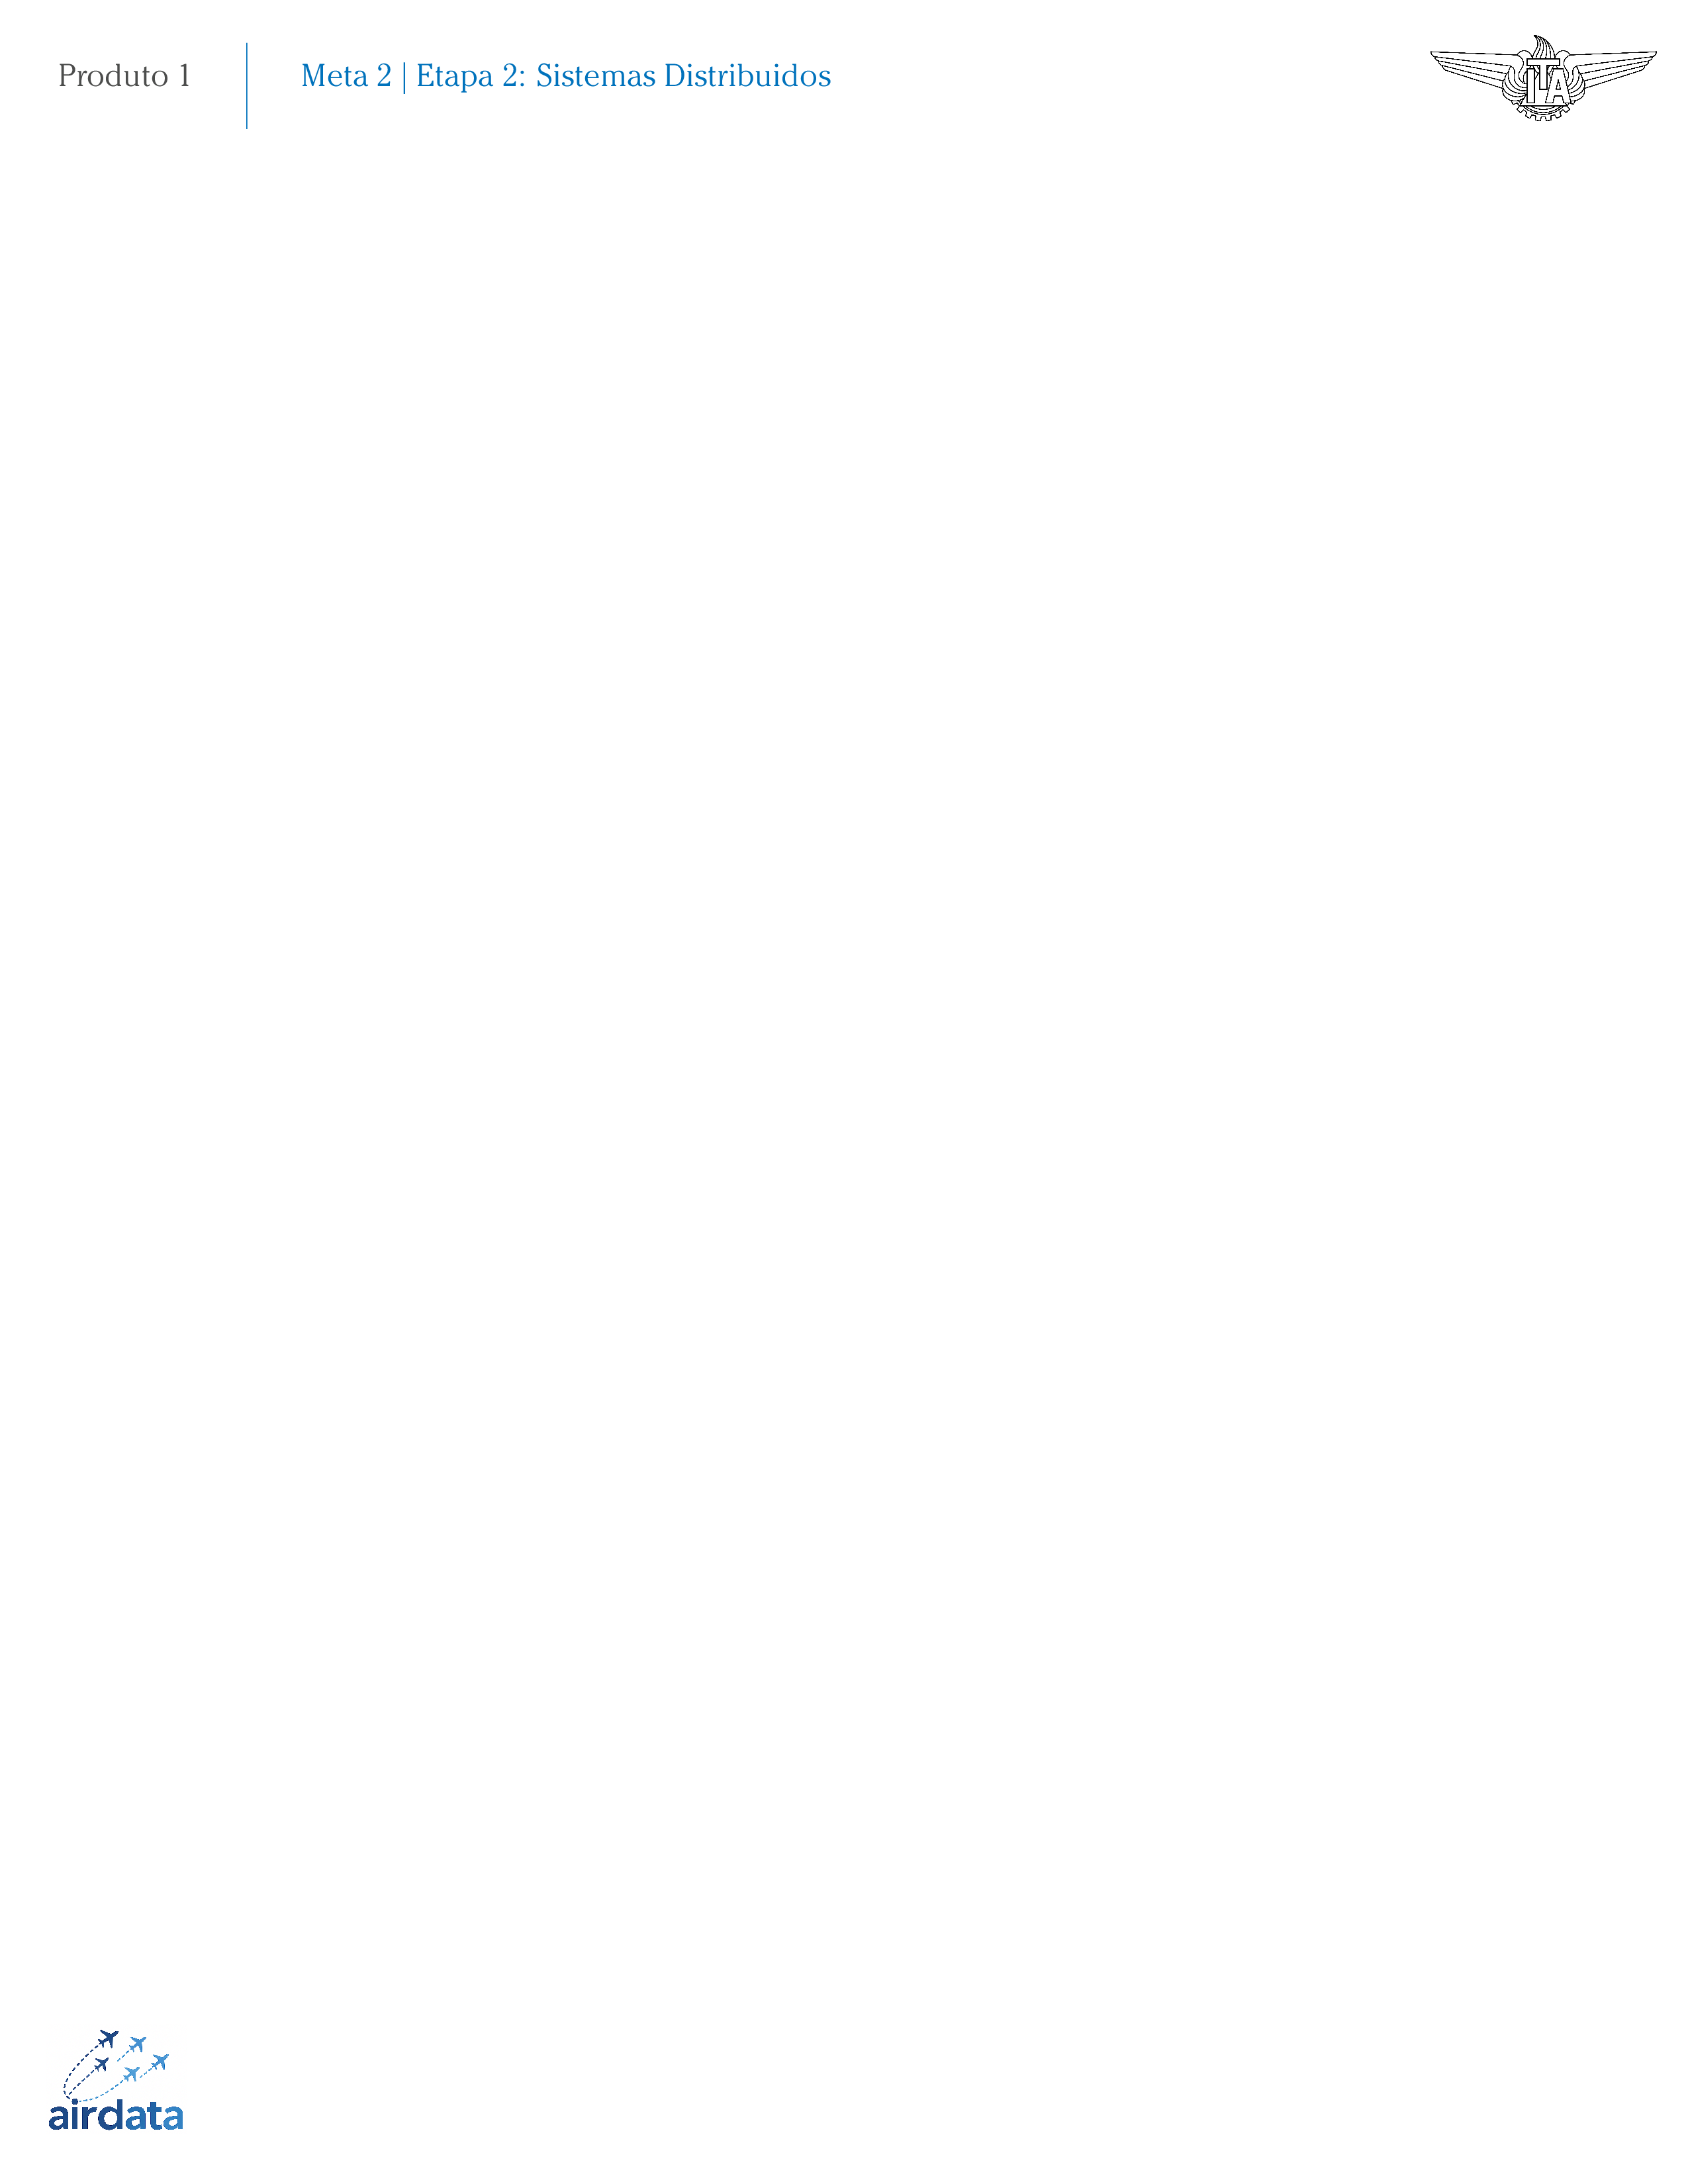
\includegraphics[width=\paperwidth,height=\paperheight]{capas/background.png}%
			\vfill
		}%
	}%
}

% Aplica a imagem de fundo em TODAS as páginas
\AddToShipoutPictureBG{\BackgroundPic}

% settings/pretextualpages.tex
% Define o background exclusivo para páginas pré-textuais

\newenvironment{pretextualblock}
{
	\ClearShipoutPictureBG
	\AddToShipoutPictureBG{
		\put(0,0){
			\parbox[b][\paperheight]{\paperwidth}{%
				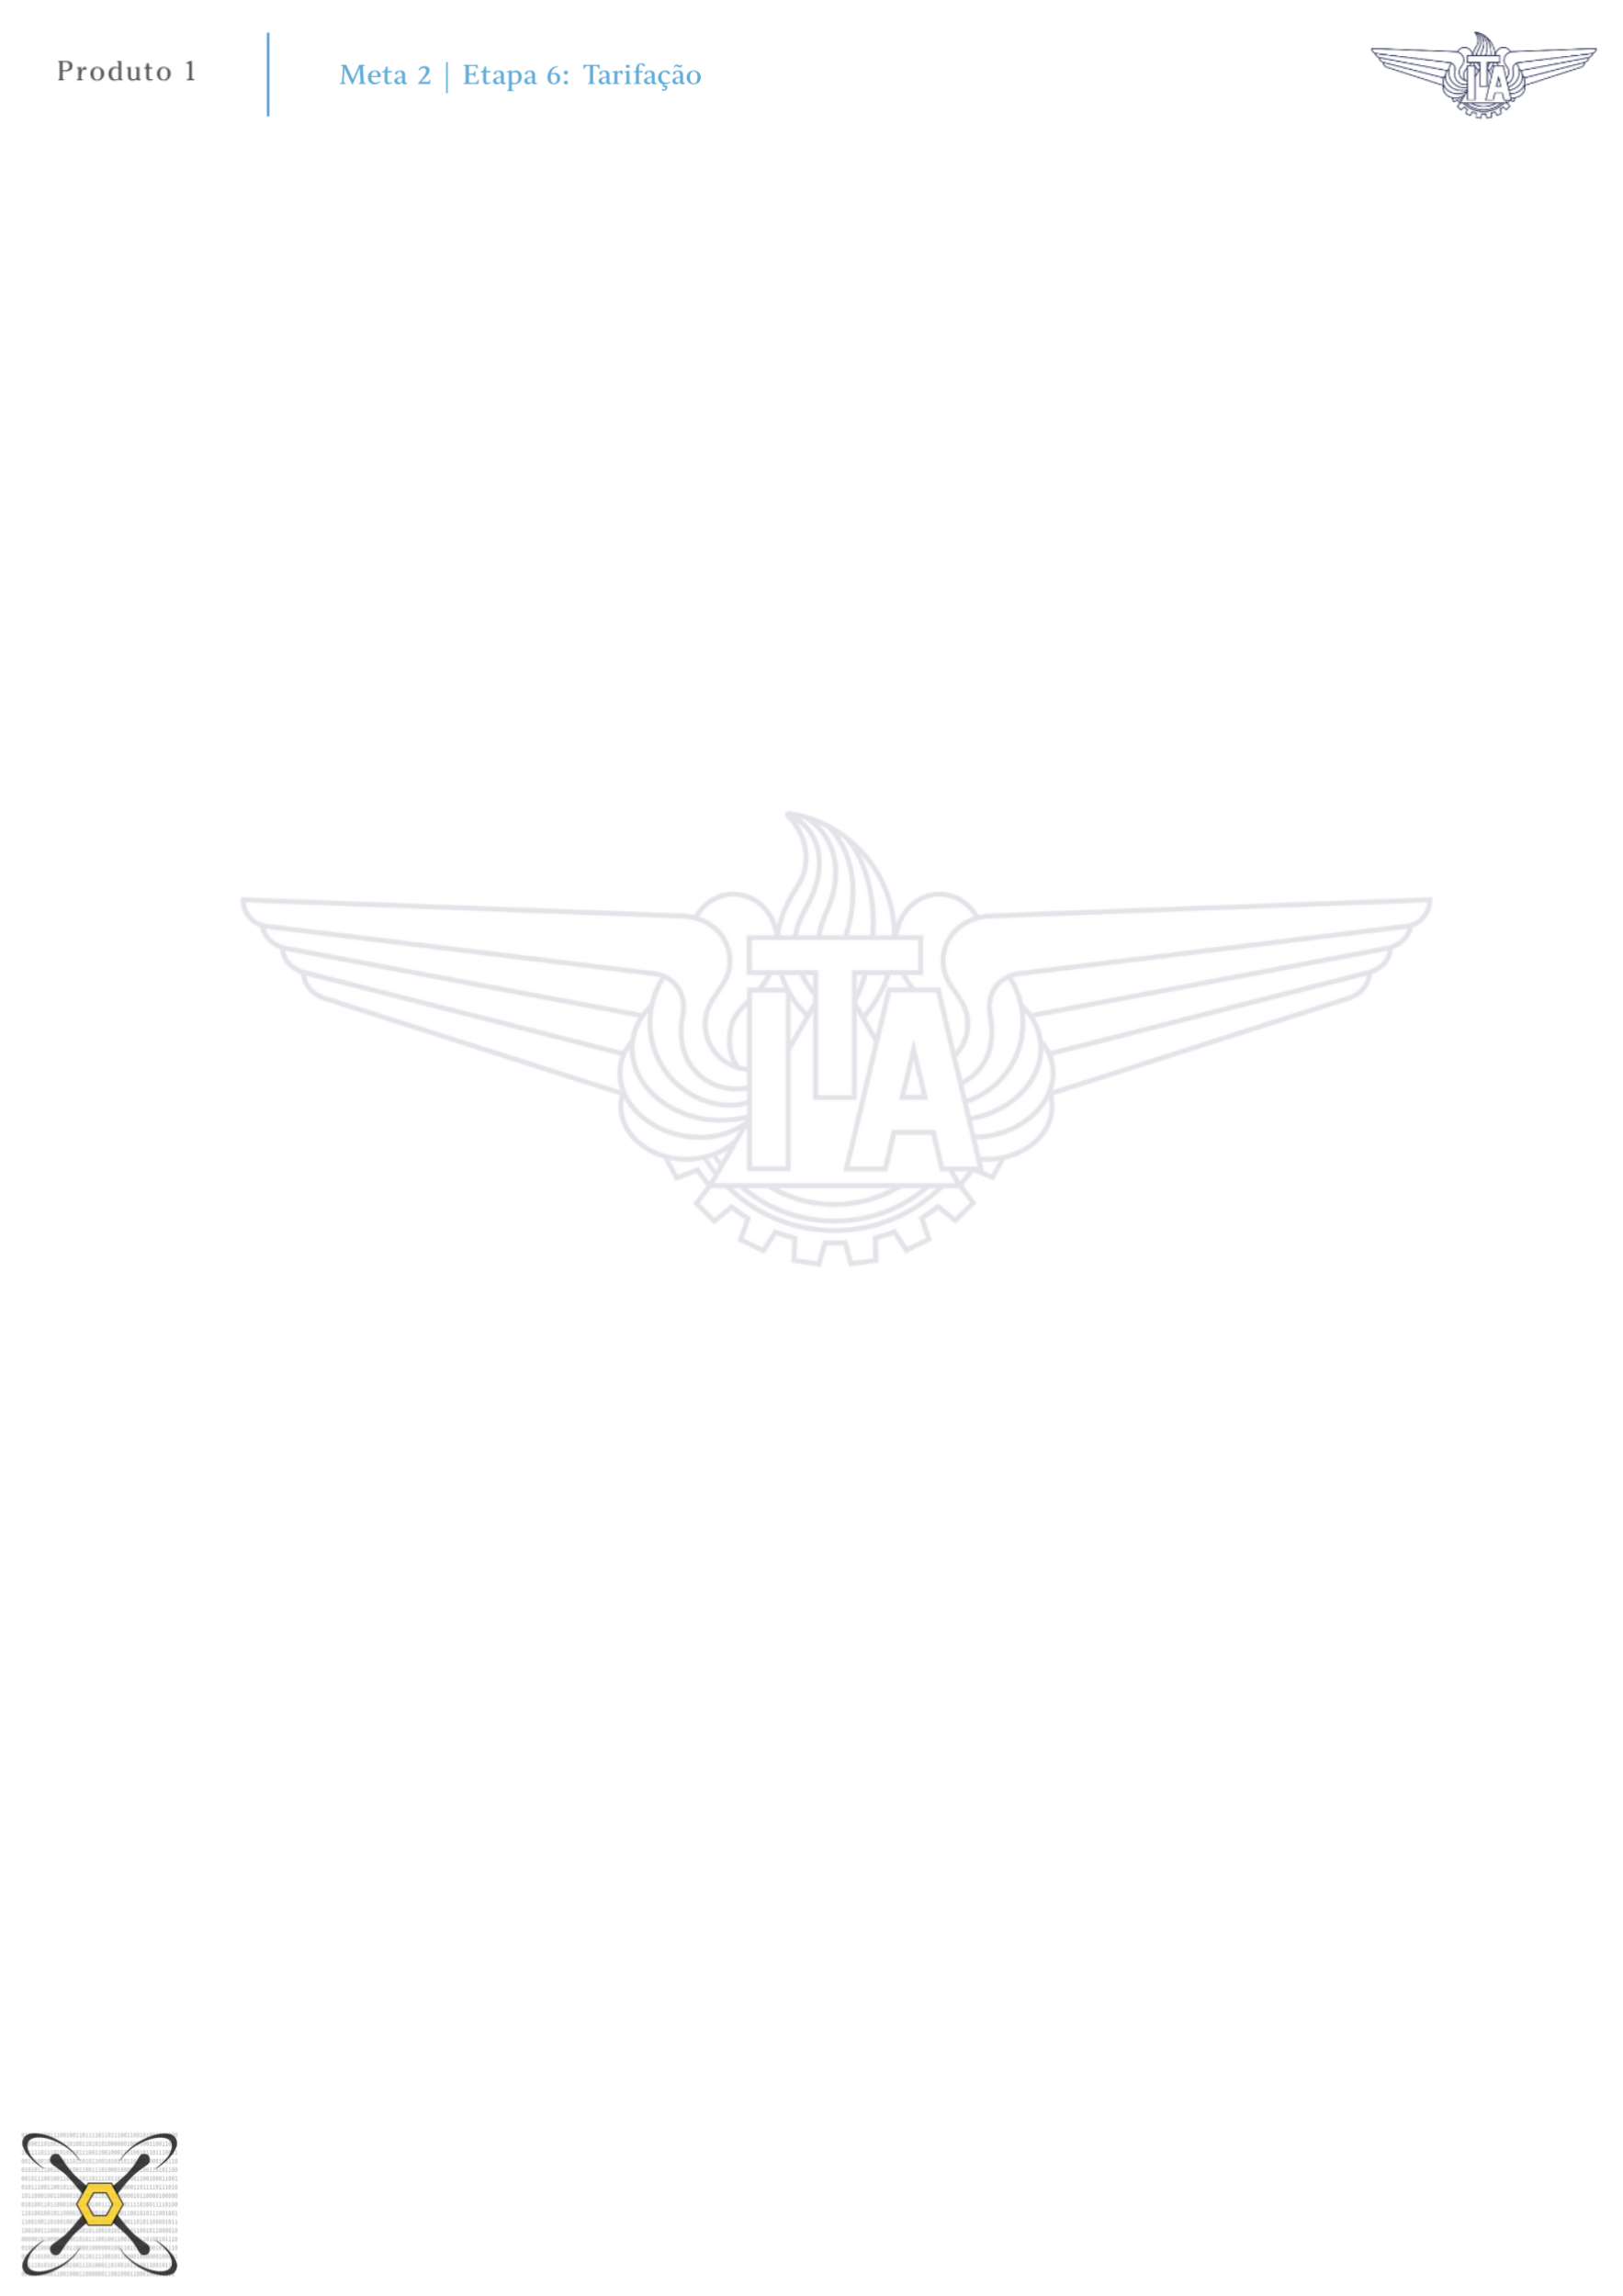
\includegraphics[width=\paperwidth,height=\paperheight]{capas/background_pretex}%
			}
		}
	}
}
{
	\input{settings/background.tex} % Restaura o background padrão
}

\end{verbatim}

Essa ordem é proposital para garantir que os pacotes e estilos sejam carregados antes dos elementos visuais como capa e plano de fundo.

\section{Sugestão de novos capítulos}

Novos arquivos podem ser adicionados à pasta \texttt{caps/} com nomes como \texttt{cap03.tex}, \texttt{cap04.tex}, etc. A inclusão no documento é feita via:

\begin{verbatim}
\chapter{Estrutura do Template}

O template TED ITA-SAC foi organizado de forma modular, para facilitar manutenção, reuso e colaboração entre diferentes autores. A estrutura principal está organizada da seguinte forma:

\section{Visão geral}

\begin{verbatim}
	.
	|- main.tex                 % Arquivo principal (documento raiz)
	|- settings/                % Configurações gerais
	|  |- background.tex        % Marca d’água e fundo
	|  |- coverpage.tex         % Página de capa
	|  |- fonts.tex             % Fonte Cheltenham
	|  |- pretextualpages.tex  % Sumário, listas, elementos iniciais
	|  |- setabnt.tex          % Estilo de citação ABNT
	|  |- setcolor.tex         % Paleta de cores do template
	|  |- setlayout.tex        % Margens, espaçamento, cabeçalho
	|  |- settitles.tex        % Estilo de títulos e capítulos
	|  \_ usepackage.tex       % Pacotes utilizados no projeto
	|- caps/                   % Capítulos do relatório
	|  |- cap00.tex            % Introdução
	|  |- cap01.tex            % Conteúdo específico
	|  \_ etc.
	|- siglas/                 % (Opcional) Siglas, glossários
	|- refs/                   % (Opcional) Arquivos .bib
	\_ Makefile                % Automação de compilação
\end{verbatim}


\section{Função de cada componente}

\begin{itemize}
    \item \texttt{main.tex}: ponto de entrada do projeto. Controla a ordem dos elementos.
    \item \texttt{settings/}: conjunto de arquivos para configurar todos os aspectos do template.
    \item \texttt{caps/}: contém os capítulos do relatório (modularizados).
    \item \texttt{siglas/}: pasta destinada ao glossário e acrônimos, caso ativado.
    \item \texttt{refs/}: local sugerido para o arquivo de bibliografia (\texttt{.bib}).
    \item \texttt{Makefile}: automatiza as etapas de compilação (XeLaTeX + BibTeX + Glossário).
\end{itemize}

\section{Ordem de carregamento no \texttt{main.tex}}

O arquivo \texttt{main.tex} importa os componentes da seguinte forma:

\begin{verbatim}
\input{settings/usepackage.tex}
\input{settings/setabnt.tex}
\input{settings/setlayout.tex}
\input{settings/fonts.tex}
\input{settings/setcolor.tex}
\input{settings/settitles.tex}
\input{settings/coverpage.tex}
\input{settings/background.tex}
\input{settings/pretextualpages.tex}
\end{verbatim}

Essa ordem é proposital para garantir que os pacotes e estilos sejam carregados antes dos elementos visuais como capa e plano de fundo.

\section{Sugestão de novos capítulos}

Novos arquivos podem ser adicionados à pasta \texttt{caps/} com nomes como \texttt{cap03.tex}, \texttt{cap04.tex}, etc. A inclusão no documento é feita via:

\begin{verbatim}
\input{caps/cap03.tex}
\end{verbatim}

Recomenda-se utilizar comandos \verb|\chapter| dentro de cada arquivo, para manter a consistência da numeração.



\end{verbatim}

Recomenda-se utilizar comandos \verb|\chapter| dentro de cada arquivo, para manter a consistência da numeração.



\end{verbatim}

Recomenda-se utilizar comandos \verb|\chapter| dentro de cada arquivo, para manter a consistência da numeração.



\end{verbatim}

Recomenda-se utilizar comandos \verb|\chapter| dentro de cada arquivo, para manter a consistência da numeração.


